% Options for packages loaded elsewhere
\PassOptionsToPackage{unicode}{hyperref}
\PassOptionsToPackage{hyphens}{url}
%
\documentclass[
]{book}
\usepackage{lmodern}
\usepackage{amssymb,amsmath}
\usepackage{ifxetex,ifluatex}
\ifnum 0\ifxetex 1\fi\ifluatex 1\fi=0 % if pdftex
  \usepackage[T1]{fontenc}
  \usepackage[utf8]{inputenc}
  \usepackage{textcomp} % provide euro and other symbols
\else % if luatex or xetex
  \usepackage{unicode-math}
  \defaultfontfeatures{Scale=MatchLowercase}
  \defaultfontfeatures[\rmfamily]{Ligatures=TeX,Scale=1}
\fi
% Use upquote if available, for straight quotes in verbatim environments
\IfFileExists{upquote.sty}{\usepackage{upquote}}{}
\IfFileExists{microtype.sty}{% use microtype if available
  \usepackage[]{microtype}
  \UseMicrotypeSet[protrusion]{basicmath} % disable protrusion for tt fonts
}{}
\makeatletter
\@ifundefined{KOMAClassName}{% if non-KOMA class
  \IfFileExists{parskip.sty}{%
    \usepackage{parskip}
  }{% else
    \setlength{\parindent}{0pt}
    \setlength{\parskip}{6pt plus 2pt minus 1pt}}
}{% if KOMA class
  \KOMAoptions{parskip=half}}
\makeatother
\usepackage{xcolor}
\IfFileExists{xurl.sty}{\usepackage{xurl}}{} % add URL line breaks if available
\IfFileExists{bookmark.sty}{\usepackage{bookmark}}{\usepackage{hyperref}}
\hypersetup{
  pdftitle={Introduction to biostatistics and machine learning},
  pdfauthor={Olga Dethlefsen, Eva Freyhult, Bengt Sennblad, Payam Emami},
  hidelinks,
  pdfcreator={LaTeX via pandoc}}
\urlstyle{same} % disable monospaced font for URLs
\usepackage{color}
\usepackage{fancyvrb}
\newcommand{\VerbBar}{|}
\newcommand{\VERB}{\Verb[commandchars=\\\{\}]}
\DefineVerbatimEnvironment{Highlighting}{Verbatim}{commandchars=\\\{\}}
% Add ',fontsize=\small' for more characters per line
\usepackage{framed}
\definecolor{shadecolor}{RGB}{248,248,248}
\newenvironment{Shaded}{\begin{snugshade}}{\end{snugshade}}
\newcommand{\AlertTok}[1]{\textcolor[rgb]{0.94,0.16,0.16}{#1}}
\newcommand{\AnnotationTok}[1]{\textcolor[rgb]{0.56,0.35,0.01}{\textbf{\textit{#1}}}}
\newcommand{\AttributeTok}[1]{\textcolor[rgb]{0.77,0.63,0.00}{#1}}
\newcommand{\BaseNTok}[1]{\textcolor[rgb]{0.00,0.00,0.81}{#1}}
\newcommand{\BuiltInTok}[1]{#1}
\newcommand{\CharTok}[1]{\textcolor[rgb]{0.31,0.60,0.02}{#1}}
\newcommand{\CommentTok}[1]{\textcolor[rgb]{0.56,0.35,0.01}{\textit{#1}}}
\newcommand{\CommentVarTok}[1]{\textcolor[rgb]{0.56,0.35,0.01}{\textbf{\textit{#1}}}}
\newcommand{\ConstantTok}[1]{\textcolor[rgb]{0.00,0.00,0.00}{#1}}
\newcommand{\ControlFlowTok}[1]{\textcolor[rgb]{0.13,0.29,0.53}{\textbf{#1}}}
\newcommand{\DataTypeTok}[1]{\textcolor[rgb]{0.13,0.29,0.53}{#1}}
\newcommand{\DecValTok}[1]{\textcolor[rgb]{0.00,0.00,0.81}{#1}}
\newcommand{\DocumentationTok}[1]{\textcolor[rgb]{0.56,0.35,0.01}{\textbf{\textit{#1}}}}
\newcommand{\ErrorTok}[1]{\textcolor[rgb]{0.64,0.00,0.00}{\textbf{#1}}}
\newcommand{\ExtensionTok}[1]{#1}
\newcommand{\FloatTok}[1]{\textcolor[rgb]{0.00,0.00,0.81}{#1}}
\newcommand{\FunctionTok}[1]{\textcolor[rgb]{0.00,0.00,0.00}{#1}}
\newcommand{\ImportTok}[1]{#1}
\newcommand{\InformationTok}[1]{\textcolor[rgb]{0.56,0.35,0.01}{\textbf{\textit{#1}}}}
\newcommand{\KeywordTok}[1]{\textcolor[rgb]{0.13,0.29,0.53}{\textbf{#1}}}
\newcommand{\NormalTok}[1]{#1}
\newcommand{\OperatorTok}[1]{\textcolor[rgb]{0.81,0.36,0.00}{\textbf{#1}}}
\newcommand{\OtherTok}[1]{\textcolor[rgb]{0.56,0.35,0.01}{#1}}
\newcommand{\PreprocessorTok}[1]{\textcolor[rgb]{0.56,0.35,0.01}{\textit{#1}}}
\newcommand{\RegionMarkerTok}[1]{#1}
\newcommand{\SpecialCharTok}[1]{\textcolor[rgb]{0.00,0.00,0.00}{#1}}
\newcommand{\SpecialStringTok}[1]{\textcolor[rgb]{0.31,0.60,0.02}{#1}}
\newcommand{\StringTok}[1]{\textcolor[rgb]{0.31,0.60,0.02}{#1}}
\newcommand{\VariableTok}[1]{\textcolor[rgb]{0.00,0.00,0.00}{#1}}
\newcommand{\VerbatimStringTok}[1]{\textcolor[rgb]{0.31,0.60,0.02}{#1}}
\newcommand{\WarningTok}[1]{\textcolor[rgb]{0.56,0.35,0.01}{\textbf{\textit{#1}}}}
\usepackage{longtable,booktabs}
% Correct order of tables after \paragraph or \subparagraph
\usepackage{etoolbox}
\makeatletter
\patchcmd\longtable{\par}{\if@noskipsec\mbox{}\fi\par}{}{}
\makeatother
% Allow footnotes in longtable head/foot
\IfFileExists{footnotehyper.sty}{\usepackage{footnotehyper}}{\usepackage{footnote}}
\makesavenoteenv{longtable}
\usepackage{graphicx}
\makeatletter
\def\maxwidth{\ifdim\Gin@nat@width>\linewidth\linewidth\else\Gin@nat@width\fi}
\def\maxheight{\ifdim\Gin@nat@height>\textheight\textheight\else\Gin@nat@height\fi}
\makeatother
% Scale images if necessary, so that they will not overflow the page
% margins by default, and it is still possible to overwrite the defaults
% using explicit options in \includegraphics[width, height, ...]{}
\setkeys{Gin}{width=\maxwidth,height=\maxheight,keepaspectratio}
% Set default figure placement to htbp
\makeatletter
\def\fps@figure{htbp}
\makeatother
\setlength{\emergencystretch}{3em} % prevent overfull lines
\providecommand{\tightlist}{%
  \setlength{\itemsep}{0pt}\setlength{\parskip}{0pt}}
\setcounter{secnumdepth}{5}
\ifluatex
  \usepackage{selnolig}  % disable illegal ligatures
\fi

\title{Introduction to biostatistics and machine learning}
\author{Olga Dethlefsen, Eva Freyhult, Bengt Sennblad, Payam Emami}
\date{2020-11-10}

\usepackage{amsthm}
\newtheorem{theorem}{Theorem}[chapter]
\newtheorem{lemma}{Lemma}[chapter]
\newtheorem{corollary}{Corollary}[chapter]
\newtheorem{proposition}{Proposition}[chapter]
\newtheorem{conjecture}{Conjecture}[chapter]
\theoremstyle{definition}
\newtheorem{definition}{Definition}[chapter]
\theoremstyle{definition}
\newtheorem{example}{Example}[chapter]
\theoremstyle{definition}
\newtheorem{exercise}{Exercise}[chapter]
\theoremstyle{remark}
\newtheorem*{remark}{Remark}
\newtheorem*{solution}{Solution}
\begin{document}
\maketitle

{
\setcounter{tocdepth}{1}
\tableofcontents
}
\hypertarget{preface}{%
\chapter*{Preface}\label{preface}}
\addcontentsline{toc}{chapter}{Preface}

This ``bookdown'' book contains teaching and learning materials prepared and used during ``Introduction to biostatistics and machine learning'' course organized by NBIS, National Bioinformatics Infrastructure Sweden. The course is open for PhD students, postdoctoral researcher and other employees in need of biostatistical skills within Swedish universities. The materials are geared towards life scientists wanting to be able to understand and use basic statistical and machine learning methods. It may also suits those already applying biostatistical methods but who have never gotten a chance to reflect on the basic statistical concepts, such as the commonly misinterpreted p-value.

More about the course \url{https://nbisweden.github.io/workshop-mlbiostatistics/}

\hypertarget{part-preliminary-mathematics}{%
\part{Preliminary Mathematics}\label{part-preliminary-mathematics}}

\hypertarget{mathematical-notations}{%
\chapter{Mathematical notations}\label{mathematical-notations}}

\textbf{Aims}

\begin{itemize}
\tightlist
\item
  to recapitulate the basic notations and conventions used in mathematics and statistics
\end{itemize}

\textbf{Learning outcomes}

\begin{itemize}
\tightlist
\item
  to recognize natural numbers, integrals and real numbers
\item
  to understand the differences between variables and constants
\item
  to use symbols, especially Sigma and product notations, to represent mathematical operations
\end{itemize}

\hypertarget{numbers}{%
\section{Numbers}\label{numbers}}

\begin{itemize}
\tightlist
\item
  \textbf{Natural numbers, N}: numbers such as 0, 1, 3, \ldots{}
\item
  \textbf{Integers, Z}: include negative numbers \ldots, -2, -1, 0, 1, 2
\item
  \textbf{Rational numbers}: numbers that can be expressed as a ratio two integers, i.e.~in a form \(\frac{a}{b}\), where \(a\) and \(b\) are integers, and \(b\neq0\)
\item
  \textbf{Real numbers, R}: include both rational and irrational numbers
\item
  \textbf{Reciprocal} of any number is found by diving 1 by the number, e.g.~reciprocal of 5 is \(\frac{1}{5}\)
\item
  \textbf{Absolute value} of a number can be viewed as its distance from zero, e.g.~the absolute value of 6 is 6, written as \(|6| = 6\) and absolute value of -5 is 5, written as \(|-5| = 5\)
\item
  \textbf{Factorial} of a non-negative integer number \(n\) is denoted by \(n!\) and it is a product of all positive integers less than or equal to \(n\), e.g.~\(4! = 4 \cdot 3\cdot 2 \cdot 1 = 24\)
\end{itemize}

\hypertarget{variables-constants-and-letters}{%
\section{Variables, constants and letters}\label{variables-constants-and-letters}}

Mathematics gives us a precise language to communicate different concepts and ideas. To be able to use it it is essential to learn symbols and understand how they are used to represent physical quantities as well as understand the rules and conventions that have been developed to manipulate them.

\begin{itemize}
\tightlist
\item
  \textbf{variables}: things that can vary, e.g.~temperature and time
\item
  \textbf{constants}: fixed and unchanging quantities used in certain calculations, e.g.~3.14159
\item
  in principle one could freely choose letters and symbols to represent variables and constants, but it is helpful and choose letters and symbols that have meaning in a particular context. Hence, we
\item
  \(x, y, z\), the end of the alphabet is reserved for variables
\item
  \(a, b, c\), the beginning of the alphabet is used to represent constants
\item
  \(\pi\), \(\omega\) and Greek letters below are used frequently used to represent common constant, e.g.~\(\pi = 3.14159\)
\end{itemize}

\begin{longtable}[]{@{}llllll@{}}
\caption{\label{tab:greek-table} Uppercase and lowercase letters of the Greek alphabet}\tabularnewline
\toprule
Letter & Upper case & Lower case & Letter & Upper case & Lower case\tabularnewline
\midrule
\endfirsthead
\toprule
Letter & Upper case & Lower case & Letter & Upper case & Lower case\tabularnewline
\midrule
\endhead
Alpha & A & \(\alpha\) & Nu & N & \(\nu\)\tabularnewline
Beta & B & \(\beta\) & Xi & \(\Xi\) & \(\xi\)\tabularnewline
Gamma & \(\Gamma\) & \(\gamma\) & Omicron & O & o\tabularnewline
Delta & \(\Delta\) & \(\delta\) & Pi & \(\Pi\) & \(\pi\)\tabularnewline
Epsilon & E & \(\epsilon\) & Rho & P & \(\rho\)\tabularnewline
Zeta & Z & \(\zeta\) & Sigma & \(\Sigma\) & \(\sigma\)\tabularnewline
Eta & H & \(\eta\) & Tau & T & \(\tau\)\tabularnewline
Theta & \(\Theta\) & \(\theta\) & Upsilon & Y & \(\upsilon\)\tabularnewline
Iota & i & \(\iota\) & Phi & \(\Phi\) & \(\phi\)\tabularnewline
Kappa & K & \(\kappa\) & Chi & \(\Gamma\) & \(\gamma\)\tabularnewline
Lambda & \(\Gamma\) & \(\gamma\) & Psi & \(\Psi\) & \(\psi\)\tabularnewline
Mu & M & \(\mu\) & Omega & \(\Omega\) & \(\omega\)\tabularnewline
\bottomrule
\end{longtable}

\hypertarget{a-precise-language}{%
\section{A precise language}\label{a-precise-language}}

\begin{itemize}
\tightlist
\item
  Mathematics is a precise language meaning that a special attention has to be paid to the exact position of any symbol in relation to other.
\item
  Given two symbols \(x\) and \(y\), \(xy\) and \(x^y\) and \(x_y\) can mean different things
\item
  \(xy\) stands for multiplication, \(x^y\) for superscript and \(x_y\) for subscript
\end{itemize}

\hypertarget{using-symbols}{%
\section{Using symbols}\label{using-symbols}}

If the letters \(x\) and \(y\) represent two numbers, then:

\begin{itemize}
\tightlist
\item
  their \textbf{sum} is written as \(x + y\)
\item
  subtracting \(y\) from \(x\) is \(x - y\), known also as \textbf{difference}
\item
  to multiply \(x\) and \(y\) we written as \(x \cdot y\) or also with the multiplication signed omitted as \(xy\). The quantity is known as \textbf{product of x and y}
\item
  multiplication is \textbf{associative}, e.g.~when we multiply three numbers together, \(x \cdot y \cdot z\), the order of multiplication does not matter, so \(x \cdot y \cdot z\) is the same as \(z \cdot x \cdot y\) or \(y cdot z \cdot x\)
\item
  division is denoted by \(\frac{x}{y}\) and mans that \(x\) is divided by \(y\). In this expression \(x\), on the top, is called \textbf{numerator} and \(y\), on the bottom, is called \textbf{denominator}
\item
  division by 1 leaves any number unchanged, e.g.~\(\frac{x}{1}=x\) and division by 0 is not allowed
\end{itemize}

Equal sign

\begin{itemize}
\tightlist
\item
  the equal sign \(=\) is used in \textbf{equations}, e.g.~\(x - 5 = 0\) or \(5x = 1\)
\item
  the equal sign \(=\) can be also used in \textbf{formulae}. Physical quantities are related through a formula in many fields, e.g.~the formula \(A=\pi r^2\) relates circle area \(A\) to its radius \(r\) and the formula \(s = \frac{d}{t}\) defines speed as distance \(d\) divided by time \(t\)
\item
  the equal sign \(=\) is also used in identities, expressions true for all values of the variable, e.g.~\((x-1)(x-1) = (x^2-1)\)
\item
  opposite to the equal sign is ``is not equal to'' sign \(\neq\), e.g.~we can write \(1+2 \neq 4\)
\end{itemize}

\textbf{Sigma and Product notation}

\begin{itemize}
\tightlist
\item
  the \(\Sigma\) notation, read as \textbf{Sigma notation}, provides a convenient way of writing longs sums, e.g.~the sum of \(x_1 + x_2 + x_3 + ... + x_{20}\) is written as \(\displaystyle \sum_{i=1}^{i=20}x_i\)
\item
  the \(\Pi\) notation, read as \textbf{Product notation}, provides a convenient way of writing longs products, e.g.~\(x_1 \cdot x_2 \cdot x_3 \cdot ... \cdot x_{20}\) is written as \(\displaystyle \prod_{i=1}^{i=20}x_i\)
\end{itemize}

\hypertarget{inequalities}{%
\section{Inequalities}\label{inequalities}}

Given any two real numbers \(a\) and \(b\) there are three mutually exclusive possibilities:

\begin{itemize}
\tightlist
\item
  \(a > b\), meaning that \(a\) is greater than \(b\)
\item
  \(a < b\), meaning that \(a\) is less than \(b\)
\item
  \(a = b\), meaning that \(a\) is equal to \(b\)
\end{itemize}

Strict and weak

\begin{itemize}
\tightlist
\item
  inequality in \(a > b\) and \(a < b\) is \textbf{strict}
\item
  as oppose to \textbf{weak} inequality denoted as \(a \ge b\) or \(a \le b\)
\end{itemize}

Some useful relations are:

\begin{itemize}
\tightlist
\item
  if \(a > b\) and \(b > c\) then \(a > c\)
\item
  if \(a > b\) then \(a + c > b\) for any \(c\)
\item
  if \(a > b\) then \(ac > bc\) for any positive \(c\)
\item
  if \(a > b\) then \(ac < bc\) for any negative \(c\)
\end{itemize}

\hypertarget{indices-and-powers}{%
\section{Indices and powers}\label{indices-and-powers}}

\begin{itemize}
\tightlist
\item
  \textbf{Indices}, also known as \textbf{powers} are convenient when we multiply a number by itself several times
\item
  e.g.~\(5 \cdot 5 \cdot 5\) is written as \(5^3\) and \(4 \cdot 4 \cdot 4 \cdot 4 \cdot 4\) is written as \(4^5\)
\item
  in the expression \(x^y\), \(x\) is called the \emph{base} and \(y\) is called \emph{index} or \emph{power}
\end{itemize}

The laws of indices state:

\begin{itemize}
\tightlist
\item
  \(a^m \cdot a^n = a^{m+n}\)
\item
  \(\frac{a^m}{a^n} = a^{m-n}\)
\item
  \((a^m)^n = a^{m\cdot n}\)
\end{itemize}

Rules derived from the laws of indices:

\begin{itemize}
\tightlist
\item
  \(a^0 = 1\)
\item
  \(a^1 = a\)
\end{itemize}

Negative and fractional indices:

\begin{itemize}
\tightlist
\item
  \(a^{-m} = \frac{1}{a^m}\) e.g.~\(5^{-2} = \frac{1}{5^2} = \frac{1}{25}\) for negative indices
\item
  e.g.~\(4^{\frac{1}{2}} = \sqrt{4}\) or \(8^{\frac{1}{3}} = \sqrt[3]{8}\) for fractional indices
\end{itemize}

\begin{center}\rule{0.5\linewidth}{0.5pt}\end{center}

\hypertarget{exercises-notations}{%
\section{Exercises: notations}\label{exercises-notations}}

\begin{exercise}
\protect\hypertarget{exr:m-notations-numbers}{}{\label{exr:m-notations-numbers} }
Classify numbers as natural, integers or real. If reall, specify if they are rational or irrational.

\begin{enumerate}
\def\labelenumi{\alph{enumi})}
\tightlist
\item
  \(\frac{1}{3}\)
\item
  2
\item
  \(\sqrt{4}\)
\item
  2.3
\item
  \(\pi\)
\item
  \(\sqrt{5}\)
\item
  -7
\item
  0
\item
  0.25
\end{enumerate}
\end{exercise}

\begin{exercise}
\protect\hypertarget{exr:m-notations-variables-constants}{}{\label{exr:m-notations-variables-constants} }Classify below descriptors as variables or constants. Do you know the letters or symbols commonly used to represent these?

\begin{enumerate}
\def\labelenumi{\alph{enumi})}
\tightlist
\item
  speed of light in vacuum
\item
  mass of an apple
\item
  volume of an apple
\item
  concentration of vitamin C in an apple
\item
  distance from Stockholm central station to Uppsala central station
\item
  time on the train to travel between the above stations
\item
  electron charge
\end{enumerate}
\end{exercise}

\begin{exercise}
\protect\hypertarget{exr:m-notations-sigma-product}{}{\label{exr:m-notations-sigma-product} }Write out explicitly what is meant by the following:

\begin{enumerate}
\def\labelenumi{\alph{enumi})}
\item
  \(\displaystyle \sum_{i=1}^{i=6}k_i\)
\item
  \(\displaystyle \prod_{i=1}^{i=6}k_i\)
\item
  \(\displaystyle \sum_{i=1}^{i=6}i^k\)
\item
  \(\displaystyle \prod_{i=1}^{i=3}i^k\)
\item
  \(\displaystyle \sum_{i=1}^{n}i\)
\item
  \(\displaystyle \sum_{i=1}^{i=4}(i + 1)^k\)
\item
  \(\displaystyle \prod_{i=1}^{i=4}(k + 1)^i\)
\item
  \(\displaystyle \prod_{i=0}^{n}i\)
\end{enumerate}
\end{exercise}

\begin{exercise}
\protect\hypertarget{exr:m-notations-sigma-product-reverse}{}{\label{exr:m-notations-sigma-product-reverse} }
Use Sigma or Product notation to represent the long sums and products below:

\begin{enumerate}
\def\labelenumi{\alph{enumi})}
\tightlist
\item
  \(1+2+3+4+5+6\)
\item
  \(2^2+3^2+4^2+5^2\)
\item
  \(4 \cdot 5 \cdot 6 \cdot 7 \cdot 8\)
\item
  \(1 + \frac{1}{2} + \frac{1}{3} + \frac{1}{4} + \frac{1}{5} +...+ \frac{1}{n}\)
\item
  \(2-2^2+2^3-2^4 + ...+2^n\)
\item
  \(3+6+9+12+···+60\)
\item
  \(3x + 6x^2 + 9x^3 + 12x^4 +...+60x^{20}\)
\item
  \(3x \cdot 6x^2 \cdot 9x^3 \cdot 12x^4 \cdot...\cdot 60x^{20}\)
\end{enumerate}
\end{exercise}

\hypertarget{answers-to-selected-exercises-notations}{%
\section*{Answers to selected exercises (notations)}\label{answers-to-selected-exercises-notations}}
\addcontentsline{toc}{section}{Answers to selected exercises (notations)}

Exr. \ref{exr:m-notations-numbers}

\begin{enumerate}
\def\labelenumi{\alph{enumi})}
\tightlist
\item
  real, rational
\item
  natural and integers, integers include natural numbers
\item
  \(\sqrt{4} = 2\) so it is a natural number and/subset of integers
\item
  real number, rational as it could be written as \(\frac{23}{10}\)
\item
  real number, irrational as it cannot be explained by a simple fraction
\item
  real number, irrational as it cannot be explained by a simple fraction
\item
  integer, non a natural number as these do not include negative numbers
\item
  natural number, although there is some argument about it as some define natural numbers as positive integers starting from 1, 2 etc. while others include 0.
\item
  real, rational number, could be written as \(\frac{25}{100}\)
\end{enumerate}

Exr. \ref{exr:m-notations-variables-constants}

\begin{enumerate}
\def\labelenumi{\alph{enumi})}
\tightlist
\item
  constant, speed of light in vacuum is a constant, denoted \(c\) with \(c=299 792 458 \frac{m}{s}\)
\item
  variable, mass of an apple is a variable, different for different apple sizes, for instance 138 grams, denoted as \(m = 100 g\)
\item
  variable, like mass volume can be different from apple to apple, denoted as \(V\), e.g.~\(V = 200 cm^3\)
\item
  variable, like volume and mass can vary, denoted as \(\rho_i\) and defined as \(\rho_i=\frac{m}{V}\). So given 6.3 milligrams of vitamin C in our example apple, we have \(\rho_i=\frac{0.0063}{2}\frac{g}{cm^3} = 0.0000315 \frac{g}{cm^3}\) concentration of vitamin D
\item
  constant, the distance between Stockholm and Uppsala is fixed; it could be a variable though if we were to consider an experiment on a very long time scale; distance is often denoted in physics as \(d\)
\item
  variable, time on the train to travel between the stations varies, often denoted as \(t\) with speed being calculated as \(s = \frac{d}{t}\)
\item
  constant, electron charge is \(e = 1.60217663\cdot10^{-19} C\)
\end{enumerate}

Exr. \ref{exr:m-notations-sigma-product}

\begin{enumerate}
\def\labelenumi{\alph{enumi})}
\item
  \(\displaystyle \sum_{i=1}^{i=6}k_i = k_1 + k_2 + k_3 + k_4 + k_5 + k_6\)
\item
  \(\displaystyle \prod_{i=1}^{i=6}k_i = k_1 \cdot k_2 \cdot k_3 \cdot k_4 \cdot k_5 \cdot k_6\)
\item
  \(\displaystyle \sum_{i=1}^{i=3}i^k = 1^k + 2^k + 3^k\)
\item
  \(\displaystyle \prod_{i=1}^{i=3}i^k = 1^k \cdot 2^k \cdot 3^k\)
\item
  \(\displaystyle \sum_{i=1}^{n}i = 1 + 2 + 3 + ... + n\) we are using dots (\ldots) to represent all the number until \(n\). Here, thanks to Gauss we can also write \(\displaystyle \sum_{i=1}^{n}i = \frac{n(n+1)}{2}\), i.e.~Gauss formula for sum of first \(n\) natural numbers
\end{enumerate}

Exr. \ref{exr:m-notations-sigma-product-reverse}

\begin{enumerate}
\def\labelenumi{\alph{enumi})}
\item
  \(1+2+3+4+5+6 = \displaystyle \sum_{k=1}^{6}k\)
\item
  \(2^2+3^2+4^2+5^2 = \displaystyle \sum_{x=2}^{5}x^2\)
\item
  \(4 \cdot 5 \cdot 6 \cdot 7 \cdot 8 = \displaystyle \prod_{x=4}^{8}x\)
\item
  \(1 + \frac{1}{2} + \frac{1}{3} + \frac{1}{4} + \frac{1}{5} + ... + \frac{1}{n} = \displaystyle \sum_{k=1}^{n}\frac{1}{k}\)
\end{enumerate}

\hypertarget{sets}{%
\chapter{Sets}\label{sets}}

\textbf{Aims}

\begin{itemize}
\tightlist
\item
  to introduce sets and basic operations on sets
\end{itemize}

\textbf{Learning outcomes}

\begin{itemize}
\tightlist
\item
  to be able to explain what a set is
\item
  to be able to construct new sets from given sets using the basic set operations
\item
  to be able to use Venn diagrams to shows all possible logical relations between two and three sets
\end{itemize}

\hypertarget{definitions}{%
\section{Definitions}\label{definitions}}

\begin{itemize}
\tightlist
\item
  \textbf{set}: a well-defined collection of distinct objects, e.g.~\(S = \{2, 4, 6\}\)
\item
  \textbf{elements}: the objects that make up the set are also known as \textbf{elements} of the set
\item
  if \(x\) is an element of \(S\), we say that \(x\) belongs to \(S\) and write \(x \in S\) and if \(x\) is not an element of \(S\) we say that \(x\) does not belong to \(S\) and write \(x \notin S\)
\item
  a set may contain \textbf{finitely} many or \textbf{infinitely} many elements
\end{itemize}

\begin{itemize}
\tightlist
\item
  \textbf{subset, \(\subseteq\)}: if every element of set A is also in B, then A is said to be a subset of B, written as \(A \subseteq B\) and pronounced A is contained in B, e.g.~\(A \subseteq B\), when \(A = \{2, 4, 6\}\) and \$ = \(B = \{2, 4, 6, 8, 10\}\). Every set is a subset if itself.
\item
  \textbf{superset}: for our outs \(A\) and \(B\) we can also say that \(B\) is a \textbf{superset} of \(A\) and write \(B \supset A\)
\end{itemize}

\begin{itemize}
\tightlist
\item
  \textbf{cardinality}: the number of elements within a set \(S\), denoted as \(|S|\)
\item
  \textbf{empty set, \(\emptyset\)}: is a unique set with no members, denoted by \(E = \emptyset\) or \(E = \{\}\). The empty set is a subset of very set.
\end{itemize}

\hypertarget{basic-set-operations}{%
\section{Basic set operations}\label{basic-set-operations}}

\begin{itemize}
\tightlist
\item
  \textbf{union of two sets, \(\cup\) }: two sets can be ``added'' together, the union of A and B, written as \(A \cup B\), e.g.~\(\{1, 2\} \cup \{2, 3\} = \{1, 2, 3\}\) or \(\{1, 2, 3\} \cup \{1, 4, 5, 6\} = \{1, 2, 3, 4, 5, 6\}\)
\item
  \textbf{intersection of two sets, \(\cap\)}: a new set can be constructed by taking members of two sets that are ``in common'', written as \(A \cap B\), e.g.~\(\{1, 2, 3, 4, 5, 6\} \cap \{2, 3, 7\} = \{2, 3\}\) or \(\{1, 2, 3\} \cap \{7 \} = \{\emptyset \}\)
\end{itemize}

\begin{itemize}
\tightlist
\item
  \textbf{complement of a set, \(A'\), \(A^c\)}: are the elements not in A
\item
  \textbf{difference of two sets, \(\setminus\)}: two sets can be ``substracted'', denoted by \(A \setminus B\), by taking all elements that are members of A but are not members of B, e.g.~\(\{1, 2, 3, 4\} \setminus \{1, 3\} = \{2, 4\}\). This is also in other words a relative complement of A with respect to B.
\end{itemize}

\begin{itemize}
\tightlist
\item
  \textbf{partition of a set}: a partition of a set S is a set of nonempty subset of S, such that every element x in S is in exactly one of these subsets. That is, the subset are pairwise \emph{disjoint}, meaning no two sets of the partition contain elements in common, and the union of all the subset of the partition is S, e.g.~Set \(\{1, 2, 3\}\) has five partitions: i) \(\{1\}, \{2\}, \{3\}\), ii) \(\{1, 2\}, \{3\}\), iii) \(\{1,3\}, \{2\}\), iv) \(\{1\}, \{2, 3\}\) and v) \(\{1,2,3\}\)
\end{itemize}

\hypertarget{venn-diagrams}{%
\section{Venn diagrams}\label{venn-diagrams}}

Venn diagram is a diagram that shows all possible logical relations between a finite collection of different sets. A Venn diagrams shows elements as points in the plane, and sets as regions inside closed curves. A Venn diagram consists of multiple overlapping closed curves, usually circles, each representing a set.

E.g. given \(A = \{1, 2, 5\}\) and \(B = \{1, 6\}\) Venn diagram of \(A\) and \(B\):

\begin{center}\includegraphics{102-math-sets_files/figure-latex/unnamed-chunk-2-1} \end{center}

And given \(A = \{1, 2, 5\}\), \(B = \{1, 6\}\) and \(C= \{4, 7\}\) Venn diagram of \(A\), \(B\) and \(C\):

\begin{center}\includegraphics{102-math-sets_files/figure-latex/unnamed-chunk-3-1} \end{center}

And given \(A = \{1, 2, 3, 4, 5, 6\}\) and \(B= \{2, 4, 6\}\) Venn diagram of \(A\) and \(B\):

\begin{center}\includegraphics{102-math-sets_files/figure-latex/unnamed-chunk-4-1} \end{center}

\begin{center}\rule{0.5\linewidth}{0.5pt}\end{center}

\hypertarget{exercises-sets}{%
\section{Exercises: sets}\label{exercises-sets}}

\begin{exercise}
\protect\hypertarget{exr:m-sets-01}{}{\label{exr:m-sets-01} }
Given set \(S = \{1, 2, 3, 4, 5, 6\}\):

\begin{enumerate}
\def\labelenumi{\alph{enumi})}
\tightlist
\item
  what is the subset \(T\) of \(S\) consisting of its even elements?
\item
  what is the complement \(T^c\)?
\item
  what is the subset \(U\) of \(S\) containing of the prime numbers in \(S\)?
\item
  what is the intersection \(T \cap U\)?
\item
  what is the union of \(T \cup U\)?
\item
  what is the set difference \(U \setminus T\)?
\end{enumerate}
\end{exercise}

\begin{exercise}
\protect\hypertarget{exr:m-sets-02}{}{\label{exr:m-sets-02} }
Given set \[A = \{cat, elephant, dog, turtle, goldfish, hamster, parrot, tiger, guinea pig, lion\}\]

\begin{enumerate}
\def\labelenumi{\alph{enumi})}
\tightlist
\item
  what is the subset \(D\) of \(A\) consiting of domesticated animals?
\item
  what is the subset \(C\) of \(A\) consiting of Felidae (cat) family?
\item
  what is the interection of \(D\) and \(C\)?
\item
  what is the complement of \(D\), \(D^c\)?
\item
  what is the union of \(D\) and \(C\)?
\item
  what is the set difference of \(A \setminus C\)?
\item
  can you draw Venn diagram showing relationship between \(D\) and \(C\)?
\end{enumerate}
\end{exercise}

\hypertarget{answers-to-selected-exercises-sets}{%
\section*{Answers to selected exercises (sets)}\label{answers-to-selected-exercises-sets}}
\addcontentsline{toc}{section}{Answers to selected exercises (sets)}

Exr. \ref{exr:m-sets-01}

\begin{enumerate}
\def\labelenumi{\alph{enumi})}
\tightlist
\item
  \(T = \{2, 4, 6\}\)
\item
  \(T^c = \{1, 3, 5\}\), i.e.~\(T^c\) contains all the elements of \(S\) not in \(T\)
\item
  \(U = \{2, 3, 5\}\), the primes in \(S\)
\item
  \(T \cap U = \{2\}\), common elements of \(T\) and \(U\), i.e.~the even and prime numbers
\item
  \(T \cup U = \{2, 3, 4, 5, 6\}\)
\item
  \(U \setminus T = \{3, 5\}\), consisting of the elements of \(U\) that are not in \(T\)
\end{enumerate}

\hypertarget{functions}{%
\chapter{Functions}\label{functions}}

\textbf{Aims}

\begin{itemize}
\tightlist
\item
  to revisit the concept of a function
\end{itemize}

\textbf{Learning outcomes}

\begin{itemize}
\tightlist
\item
  to be able to explain what function, function domain and function range are
\item
  to be able to identify input, output, argument, independent variable, dependent variable
\item
  to be able to evaluate function for a given value and plot the function
\end{itemize}

\hypertarget{definitions}{%
\section{Definitions}\label{definitions}}

\begin{figure}

{\centering 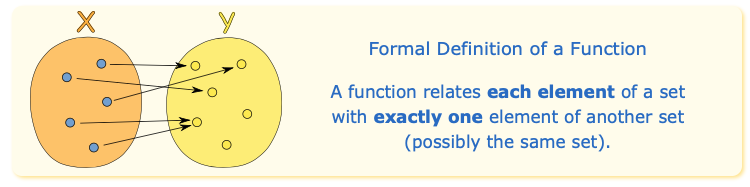
\includegraphics{figures/precourse/math-functions-definition} 

}

\caption{Formal function defition}\label{fig:func-def}
\end{figure}

\begin{itemize}
\tightlist
\item
  A \textbf{function}, \(f(x)\), can be viewed as a rule that relates input \(x\) to an output \(f(x)\)
\item
  In order for a rule to be a function it must produce a single output for any given input
\item
  Input \(x\) is also known as \textbf{argument} of the function
\item
  \textbf{Domain of a function}: the set of all values that the function ``maps''
\item
  \textbf{Range}: the set of all values that the function maps into
\end{itemize}

\textbf{Many names are used interchangeably}

Functions have been around for a while and there are many alternative names and writing conventions are being used. Common terms worth knowing:

\begin{figure}

{\centering 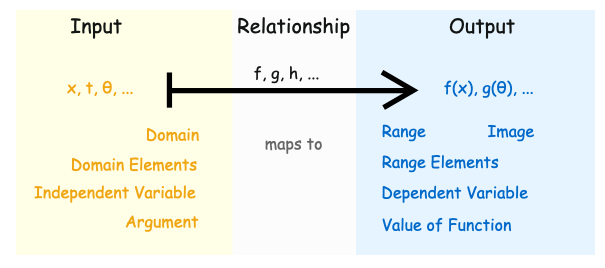
\includegraphics{figures/precourse/math-functions-terms} 

}

\caption{Common function terms}\label{fig:func-ters}
\end{figure}

\hypertarget{evaluating-function}{%
\section{Evaluating function}\label{evaluating-function}}

To evaluate a function is to replace (substitute) its variable with a given number or expression. E.g. given a rule (function) that maps temperature measurements from Celsius to Fahrenheit scale:
\[f(x) = 1.8x + 32\]
where \(x\) is temperature measurements in Celsius and \(f(x)\) is the associated value in Fahrenheit, we can find for a given temperature in Celsius corresponding temperature in Fahrenheit. Let's say we measure 10 Celsius degrees one autumn day in Uppsala and we want to share this information with a friend in USA. We can find the equivalent temperature in Fahrenheit by evaluating our function at 10, \(f(10)\), giving us \[f(10) = 1.8\cdot 10 + 32 = 50\]

\hypertarget{plotting-function}{%
\section{Plotting function}\label{plotting-function}}

Function graphs are a convenient way of showing functions, by looking at the graph it is easier to notice function's properties, e.g.~for which input values functions yields positive outcomes or whether the function is increasing or decreasing. To graph a function, one can start by evaluating function at different values for the argument \(x\) obtaining \(f(x)\), plotting the points by plotting the pairs \((x, f(x))\) and connecting the dots. E.g. evaluating our above temperature rule at -20, -10, 0, 10, 20, 30 Celsius degrees results in:

\begin{longtable}[]{@{}ccc@{}}
\toprule
x (Celsius degrees) & evaluates & f(x) (Farenheit degress)\tabularnewline
\midrule
\endhead
-20 & \(f(-20) = 1.8 \cdot (-20) + 32\) & -4\tabularnewline
-10 & \(f(-20) = 1.8 \cdot (-10) + 32\) & 14\tabularnewline
0 & \(f(-20) = 1.8 \cdot (0) + 32\) & 32\tabularnewline
10 & \(f(-20) = 1.8 \cdot (10) + 32\) & 50\tabularnewline
20 & \(f(-20) = 1.8 \cdot (20) + 32\) & 68\tabularnewline
20 & \(f(-20) = 1.8 \cdot (30) + 32\) & 86\tabularnewline
\bottomrule
\end{longtable}

\begin{figure}

{\centering \includegraphics{103-math-functions_files/figure-latex/unnamed-chunk-2-1} 

}

\caption{Graph of f(x) for the temeprature rule}\label{fig:unnamed-chunk-2}
\end{figure}

\hypertarget{standard-classes-of-functions}{%
\section{Standard classes of functions}\label{standard-classes-of-functions}}

\textbf{Algebraic function}: functions that can be expressed as the solution of a polynomial equation with integer coefficients, e.g.~

\begin{itemize}
\tightlist
\item
  constant function \(f(x) = a\)
\item
  identity function \(f(x) = x\)
\item
  linear function \(f(x) = ax + b\)
\item
  quadratic function \(f(x) = a + bx + cx^2\)
\item
  cubic function \(fx() = a + bx + cx^2 + dx^3\)
\end{itemize}

\textbf{Transcedental functions}: functions that are not algebraic, e.g.~

\begin{itemize}
\tightlist
\item
  exponential function \(f(x) = e^x\)
\item
  logarithimic function \(f(x) = log(x)\)
\item
  trigonometric function \(f(x) = -3sin(2x)\)
\end{itemize}

\begin{figure}

{\centering \includegraphics{103-math-functions_files/figure-latex/unnamed-chunk-3-1} 

}

\caption{Examples of the standard classess of functions}\label{fig:unnamed-chunk-3}
\end{figure}

\hypertarget{piecewise-functions}{%
\section{Piecewise functions}\label{piecewise-functions}}

A function can be in pieces, i.e.~we can create functions that behave differently based on the input \(x\) value. They are useful to describe situations in w which a rule changes as the input value crosses certain ``boundaries''. E.g. a function value could be fixed in a given range and equal to the input value (identify function) for input values outside this range

\begin{equation}
    f(x) =
    \left\{
        \begin{array}{cc}
                2 & \mathrm{if\ } x \le 1 \\
                x & \mathrm{if\ } x>1 \\
        \end{array}
    \right.
\end{equation}

The function can be split in many pieces, e.g.~the personal training fee in SEK may depend whether the personal trainer is hired for an hour, two hours or three or more hours:
\begin{equation}
    f(h) =
    \left\{
        \begin{array}{cc}
                500  & \mathrm{if\ } h \le 1 \\
                750  & \mathrm{if\ } 1 < h \le 2 \\
                500 + 250 \cdot h & \mathrm{if\ } h > 2 \\
        \end{array}
    \right.
\end{equation}

\begin{figure}

{\centering \includegraphics{103-math-functions_files/figure-latex/unnamed-chunk-4-1} 

}

\caption{Examples of piece-wise functions}\label{fig:unnamed-chunk-4}
\end{figure}

\begin{center}\rule{0.5\linewidth}{0.5pt}\end{center}

\hypertarget{exercises-functions}{%
\section{Exercises: functions}\label{exercises-functions}}

\begin{exercise}
\protect\hypertarget{exr:m-functions-evaluate-01}{}{\label{exr:m-functions-evaluate-01} }
Given the function for the personal trainer costs:

\begin{equation}
    f(h) =
    \left\{
        \begin{array}{cc}
                500  & \mathrm{if\ } h \le 1 \\
                750  & \mathrm{if\ } 1 < h \le 2 \\
                500 + 250 \cdot h & \mathrm{if\ } h > 2 \\
        \end{array}
    \right.
\end{equation}

How much would you pay

\begin{enumerate}
\def\labelenumi{\alph{enumi})}
\tightlist
\item
  for a 4-hours session? Evaluate function f(h) for value 4.
\item
  for a 2-hour session? Evalue function f(h) for value 2.
\end{enumerate}
\end{exercise}

\begin{exercise}
\protect\hypertarget{exr:m-functions-write}{}{\label{exr:m-functions-write} }
A museum charges 50 SEK per person for a guided tour with a group of 1 to 9 people or a fixed 500 SEK fee for a group of 10 or more people. Write a function relating the number of people \(n\) to the cost \(C\).
\end{exercise}

\begin{exercise}
\protect\hypertarget{exr:m-functions-plot-evaluate}{}{\label{exr:m-functions-plot-evaluate} }
Given function

\begin{equation}
    f(x) =
    \left\{
        \begin{array}{cc}
                x^2  & \mathrm{if\ } x \le 1 \\
                3  & \mathrm{if\ } 1 < x \le 2 \\
                x & \mathrm{if\ } x > 2 \\
        \end{array}
    \right.
\end{equation}

\begin{enumerate}
\def\labelenumi{\alph{enumi})}
\tightlist
\item
  sketch a graph of a function for \(x \in (-4, 4)\), i.e.. for \(x\) between -4 and 4
\item
  evaluate function at f(1)
\item
  evaluate function at f(4)
\end{enumerate}
\end{exercise}

\hypertarget{answers-to-selected-exercises-functions}{%
\section*{Answers to selected exercises (functions)}\label{answers-to-selected-exercises-functions}}
\addcontentsline{toc}{section}{Answers to selected exercises (functions)}

Exr. \ref{exr:m-functions-evaluate-01}

\begin{enumerate}
\def\labelenumi{\alph{enumi})}
\tightlist
\item
  \(f(4) = 500 + 250 \cdot 4 = 1500\)
\item
  \(f(2) = 750\) as \(h \le 2\) means less or equal to 2, that is including 2
\end{enumerate}

\hypertarget{differentiation}{%
\chapter{Differentiation}\label{differentiation}}

\textbf{Aims}

\begin{itemize}
\tightlist
\item
  introduce the concept of differentiation and rules of differentiation
\end{itemize}

\textbf{Learning outcomes}

\begin{itemize}
\tightlist
\item
  to be able to explain differentiation in terms of rate of change
\item
  to be able to find derivatives in simple cases
\end{itemize}

\hypertarget{rate-of-change}{%
\section{Rate of change}\label{rate-of-change}}

\begin{itemize}
\tightlist
\item
  We are often interested in the rate at which some variable is changing, e.g.~we may be interested in the rate at which the temperature is changing or the rate of water levels increasing
\item
  Rapid or unusual changes may indicate that we are dealing with unusual situations, e.g.~global warming or a flood
\item
  Rates of change can be positive, negative or zero corresponding to a variable increasing, decreasing and non-changing
\end{itemize}

\begin{figure}

{\centering 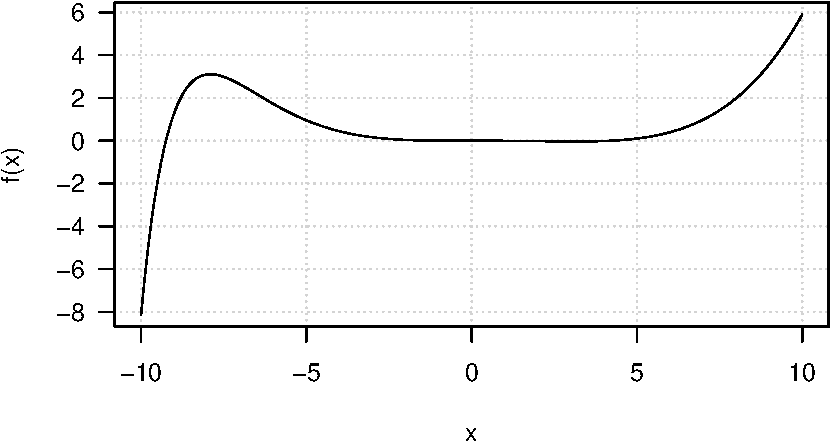
\includegraphics{104-math-differentiation_files/figure-latex/diff-rate-1} 

}

\caption{The function $f(x)$ changes at different rates for different values of $x$}\label{fig:diff-rate}
\end{figure}

The function \(f(x) = x^4 - 4x^3 - x^2 - e^{-x}\) changes at different rates for different values of \(x\), e.g.~

\begin{itemize}
\tightlist
\item
  between \(x \in (-10, -9)\) the \(f(x)\) is increasing at slightly higher pace than \(x \in (5,6)\)
\item
  between \(x \in (-7, -5)\) the \(f(x)\) is decreasing and
\item
  between \(x \in (0, 1)\) the \(f(x)\) is not changing
\item
  to be able to talk more precisely about the rate of change than just saying ``large and positive'' or ``small and negative'' change we need to quantify the changes, i.e.~assign the rate of change an exact value
\item
  \textbf{Differentiation} is a technique for calculating the rate of change of any function
\end{itemize}

\hypertarget{average-rate-of-change-across-an-interval}{%
\section{Average rate of change across an interval}\label{average-rate-of-change-across-an-interval}}

\begin{figure}

{\centering 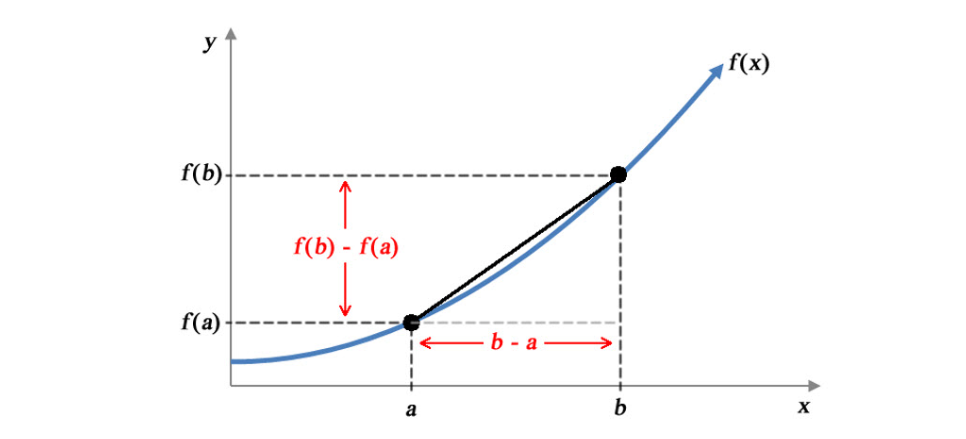
\includegraphics{figures/precourse/math-differentiation-01} 

}

\caption{The average rate of change of $f(x)$ with respect to $x$ over $[a, b]$ is equal to the slope of the secant line (in black)}\label{fig:diff-01}
\end{figure}

To dive further into calculating the rate of change let's look at Figure \ref{fig:diff-01} and define the \emph{average rate of change} of a function across an interval. Figure \ref{fig:diff-01} shows a function \(f(x)\) with two possible argument values \(a\) and \(b\) marked and their corresponding function values \(f(a)\) and \(f(b)\).

Consider that \(x\) is increasing from \(a\) to \(b\). The change in \(x\) is \(b-a\), i.e.~as \(x\) increases from \(a\) to \(b\) the function \(f(x)\) increase from \(f(a)\) to \(f(b)\). The change in \(f(x)\) is \(f(b)-f(a)\) and the average rate of change of \(y\) across the \([a,b]\) interval is:

\begin{equation}
\frac{change\:in\:y}{change\:in\:x}=\frac{f(b)-f(a)}{b-a}
\label{eq:diff-point}
\end{equation}

E.g. let's take a quadratic function \(f(x)=x^2\) and calculate the average rate of change across the interval \([1, 4]\).

\begin{itemize}
\tightlist
\item
  The change in \(x\) is \(4-1\) and the change in \(f(x)\) is \(f(4) - f(1) = 4^2 -1^2 = 16 - 1 = 15\). So the average rate of change is \(\frac{15}{3}=5\). What does this mean? It means that across the interval \([1,4]\) on average the \(f(x)\) value increases by 5 for every 1 unit increase in \(x\).
\item
  If we were to look at the average rate of change across the interval \([-2, 0]\) we would get \(\frac{f(0)-f(-2)}{0 - (-2)}=\frac{0 - (-2)^2}{2}=\frac{-4}{2} = -2\). Here, over the \([-2, 0]\) on average the \(f(x)\) value decreases by 2 for every 1 unit increase in \(x\).
\item
  Looking at the graph of \(f(x)=x^2\) verifies our calculations
\end{itemize}

\begin{figure}

{\centering 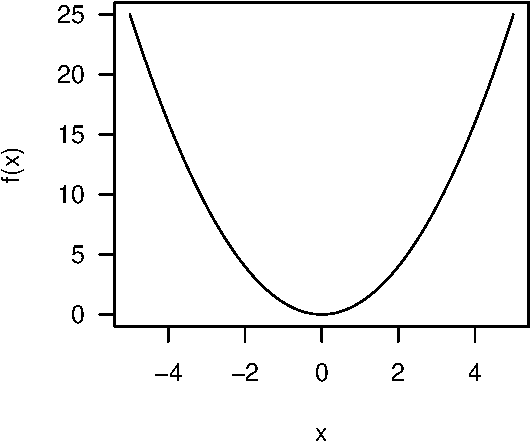
\includegraphics{104-math-differentiation_files/figure-latex/diff-avg-rate-1} 

}

\caption{Example function $f(x) = x^2$}\label{fig:diff-avg-rate}
\end{figure}

\hypertarget{rate-of-change-at-a-point}{%
\section{Rate of change at a point}\label{rate-of-change-at-a-point}}

\begin{itemize}
\tightlist
\item
  We often need to know the rate of change of a function at a point, and not simply an average rate of change across an interval.
\item
  Figure \ref{fig:diff-02}, similar to Figure \ref{fig:diff-01}, shows, instead of two points \(a\) and \(b\), point \(a\) and a second point defined in terms of its distance from the first point \(a\). Thus, the two points are now \(a\) and \(a + h\) and the distance between the two points is equal to \(h\).
\item
  Now we can write that:
  \[\frac{change\:in\:y}{change\:in\:x}=\frac{f(a+h)-f(a)}{a+h-a} = \frac{f(a+h)-f(a)}{h}\]
\end{itemize}

\begin{figure}

{\centering 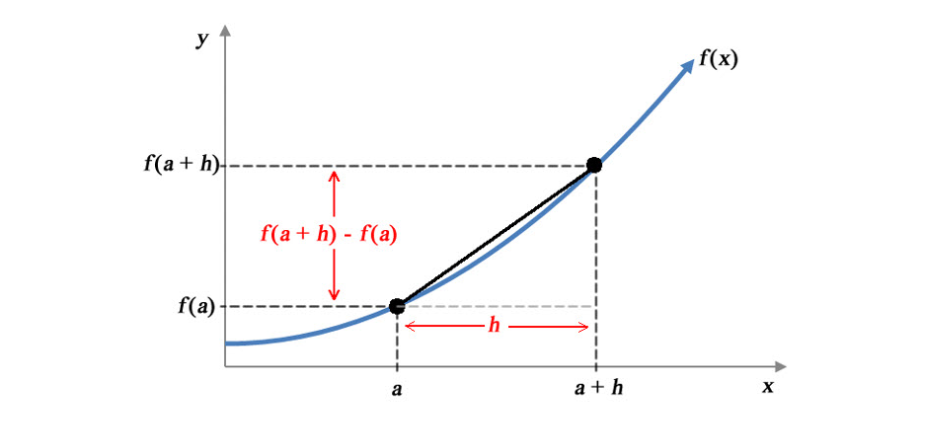
\includegraphics{figures/precourse/math-differentiation-02} 

}

\caption{The average rate of change of $f(x)$ with respect to $x$ over $[a, b]$ is equal to the slope of the secant line (in black)}\label{fig:diff-02}
\end{figure}

Further:

\begin{itemize}
\tightlist
\item
  if we assume that the second point \(a+h\) is really close to \(a\), meaning that \(h\) approaches 0, denoted as \(h \rightarrow 0\), we can find the rate of change at the point \(a\)
\item
  the distance between the two points \(a\) and \(a+h\) is getting smaller and so is the difference of the function values \(f(a+h) - f(a)\). We denote these small differences as \(\delta x\) and \(\delta y\), pronounced ``delta x'' and ``delta y'', respectively.
\item
  the term \(\delta\) reads as ``delta'' and represents a small change
\end{itemize}

We can thus continue and write that a \textbf{rate of change of a function at a point} is given by
\begin{equation}
\frac{small\:change\:in\:y}{small\:change\:in\:x} = \lim_{h\to0}\frac{f(a+h)-f(a)}{h}
\label{eq:diff-point}
\end{equation}

E.g. let's look at the linear function \(f(x) = 2x+3\). We can find the rate of change at any point of \(x\) by:
\[\frac{small\:change\:in\:y}{small\:change\:in\:x} = \\\frac{f(x+h)-f(x)}{x+h-x}= \lim_{h\to0}\frac{2(x+h)+3-(2x+3)}{x+h-x}=\lim_{h\to0}\frac{2h}{h}=2\]
It means that the function value \(f(x)\) increases by 2 for every small increase, \(h\), in \(x\). Here, this increase is the same for all the values of \(x\), i.e.~it does not depend on \(x\). \textbf{The change in function value \(f(x)\) can depend} on the value of \(x\), for instance if we look at the quadratic \(f(x)=x^2\) function, we get:
\[\frac{small\:change\:in\:y}{small\:change\:in\:x} = \\ \frac{f(x+h)-f(x)}{x+h-x}=\lim_{h\to0}\frac{x^2+2xh+h^2-x^2}{h}=\lim_{h\to0}\frac{2xh+h^2}{h}=2x+h\]
This means that:

\begin{itemize}
\tightlist
\item
  the rate of change for the function \(f(x)\) at a point \(x\) is \(2x\)
\item
  the \(f(x)\) value increases by \(2x\) for every small increase, \(h\), in \(x\)
\item
  the rate of change along a quadratic function is changing constantly according to the value of \(x\) we are looking at, it is a function of \(x\)
\item
  and finally that the rate of change does not give us any information about the rate of change globally.
\end{itemize}

\hypertarget{terminology-and-notation}{%
\section{Terminology and notation}\label{terminology-and-notation}}

\begin{itemize}
\tightlist
\item
  \textbf{differentiation} is the process of finding the rate of change of a given function
\item
  the function is said to be \textbf{differentiated}
\item
  the rate of change of a function is also known as the \textbf{derivative} of the function
\item
  given a function \(f(x)\) we say that we differentiate function in respect to \(x\) and write:
\end{itemize}

\[\lim_{h\to0}\frac{\delta y}{\delta x}= \frac{dy}{dx}\]

or use the ``prime'' \[f´(x)\]

\hypertarget{table-of-derivatives}{%
\section{Table of derivatives}\label{table-of-derivatives}}

\begin{itemize}
\tightlist
\item
  in practice, there is no need to compute \(\displaystyle \lim_{h\to0}\frac{\delta y}{\delta x}\) every time when we want to find a derivative of a function
\item
  instead, we can use patterns of the common functions and their derivatives
\end{itemize}

\begin{longtable}[]{@{}cc@{}}
\caption{\label{tab:diff-table} Common functions and their derivatives, \(k\) denotes a constant}\tabularnewline
\toprule
Function \(f(x)\) & Derivative \(f'(x)\)\tabularnewline
\midrule
\endfirsthead
\toprule
Function \(f(x)\) & Derivative \(f'(x)\)\tabularnewline
\midrule
\endhead
\(k\) & \(0\)\tabularnewline
\(x\) & \(1\)\tabularnewline
\(kx\) & \(k\)\tabularnewline
\(x^n\) & \(nx^{n-1}\)\tabularnewline
\(kx^n\) & \(knx^{n-1}\)\tabularnewline
\(e^x\) & \(e^x\)\tabularnewline
\(e^{kx}\) & \(ke^{kx}\)\tabularnewline
\(\ln(x)\) & \(\frac{1}{x}\)\tabularnewline
\(\ln(kx)\) & \(\frac{1}{x}\)\tabularnewline
\bottomrule
\end{longtable}

We can use the Table \ref{tab:diff-table} to find derivatives of some of the functions e.g.

\begin{itemize}
\tightlist
\item
  \(f(x) = 3x\), \(f'(x) = 3\)
\item
  \(f(x) = 2x^4\), \(f'(x) = 2*4x^{4-1} = 8x^3\)
\item
  \(f(x) = e^{2x}\), \(f'(x) = 2e^{2x}\)
\item
  \(f(x) = \ln(4x)\), \(f'(x) = \frac{4}{x}\)
\end{itemize}

\begin{center}\rule{0.5\linewidth}{0.5pt}\end{center}

\hypertarget{exercises-differentiation}{%
\section{Exercises (differentiation)}\label{exercises-differentiation}}

\begin{exercise}
\protect\hypertarget{exr:m-diff}{}{\label{exr:m-diff} }
\# Find derivatives of the functions

\begin{enumerate}
\def\labelenumi{\alph{enumi})}
\tightlist
\item
  \(f(x) = 2\)
\item
  \(f(x) = 2x + 1\)
\item
  \(f(x) = 5x^2\)
\item
  \(f(x) = 4x^3 + x^2\)
\item
  \(f(x) = \sqrt(x)\)
\item
  \(f(x) = \ln(2x)\)
\item
  \(f(x) = e^{x}\)
\item
  \(f(x) = \frac{9}{x^2} + ln(4x)\)
\item
  \(f(x) = 4x−6x^6\)
\item
  \(f(x) = \frac{3}{x^2}\)
\end{enumerate}
\end{exercise}

\hypertarget{answers-to-selected-exercises-differentiation}{%
\section*{Answers to selected exercises (differentiation)}\label{answers-to-selected-exercises-differentiation}}
\addcontentsline{toc}{section}{Answers to selected exercises (differentiation)}

Exr. \ref{exr:m-diff}

\begin{enumerate}
\def\labelenumi{\alph{enumi})}
\tightlist
\item
  \(f(x) = 2\), \(f'(x) = 0\)
\item
  \(f(x) = 2x + 1\), \(f'(x) = 2\)
\item
  \(f(x) = 5x^2\), \(f'(x)= 10x\)
\item
  \(f(x) = 4x^3 + x^2\), \(f'(x)=12x^2 + 2x\)
\item
  \(f(x) = \sqrt(x) = x^{\frac{1}{2}}\), \(f'(x)=\frac{1}{2}x^{\frac{1}{2}-1} = \frac{1}{2}x^{-\frac{1}{2}}\)
\item
  \(f(x) = \ln(2x)\), \(f'(x) = \frac{1}{x}\)
\item
  \(f(x) = e^{x}\), \(f'(x) = e^x\)
\end{enumerate}

\hypertarget{integration}{%
\chapter{Integration}\label{integration}}

\textbf{Aims}

\begin{itemize}
\tightlist
\item
  to introduce the concept of integration
\end{itemize}

\textbf{Learning outcomes}

\begin{itemize}
\tightlist
\item
  to be able to explain what integration is
\item
  to be able to explain the relationship between differentiation and integration
\item
  to be able to integrate simple functions
\item
  to to able to use integration to calculate the area under the curve in simple cases
\end{itemize}

\hypertarget{reverse-to-differentiation}{%
\section{Reverse to differentiation}\label{reverse-to-differentiation}}

\begin{itemize}
\tightlist
\item
  when a function \(f(x)\) is known we can differentiate it to obtain the derivative \(f'(x)\)
\item
  the reverse process is to obtain \(f(x)\) from the derivative
\item
  this process is called \textbf{integration}
\item
  apart from simple reversing differentiation integration comes very useful in finding \textbf{areas under curves}, i.e.~the area above the x-axis and below the graph of \(f(x)\), assuming that \(f(x)\) is positive
\item
  the symbol for integration is \(\int\) and is known as ``integral sign''
\end{itemize}

E.g. let's take a function \(f(x) = x^2\). Suppose we only have a derivative, which is \(f'(x) = 2x\) and we would like to find the function given this derivative. Formally we write: \[\int 2x dx = x^2 +c\]

where:

\begin{itemize}
\tightlist
\item
  the term \(2x\) within the integral is called the \textbf{integrand}
\item
  the term \(dx\) indicates the name of the variable involved, here \(x\)
\item
  \(c\) is \textbf{constant of integration}
\end{itemize}

\hypertarget{what-is-constant-of-integration}{%
\section{What is constant of integration?}\label{what-is-constant-of-integration}}

\begin{itemize}
\tightlist
\item
  Integration reverses the process of differentiation, here, given our example function \(f(x) = x^2\) that we pretended we do not know, we started with the derivative \(f´(x) = 2x\) and via integration we obtained back the very function \[\int 2x dx = x^2\]
\item
  However, many function can result in the very same derivative since the derivative of a constant is 0 e.g.~a derivatives of \(f(x) = x^2\), \(f(x) = x^2 + 10\) and \(f(x) = x^2 + \frac{1}{2}\) all equal to \(f'(x) = 2x\)
\item
  We have to take this into account when we are integrating, i.e.~reverting differentiation. As we have no way of knowing what the original function constant is, we add it in form of \(c\), i.e.~unknown constant, called the constant of integration.
\end{itemize}

\hypertarget{table-of-integrals}{%
\section{Table of integrals}\label{table-of-integrals}}

Similar to differentiation, in practice we can use tables of integrals to be able to find integrals in simple cases

\begin{longtable}[]{@{}cc@{}}
\caption{\label{tab:int-table} Common functions and their integrals, \(k\) denotes a constant}\tabularnewline
\toprule
Function \(f(x)\) & Integral \(\int f(x) dx\)\tabularnewline
\midrule
\endfirsthead
\toprule
Function \(f(x)\) & Integral \(\int f(x) dx\)\tabularnewline
\midrule
\endhead
\(constant\:k\) & \(kx + c\)\tabularnewline
\(x\) & \(\frac{x^2}{2}+c\)\tabularnewline
\(kx\) & \(k\frac{x^2}{2}+c\)\tabularnewline
\(x^n\) & \(\frac{x^{n+1}}{n+1}+c\;\; if\;n\neq-1\)\tabularnewline
\(kx^n\) & \(k\frac{x^{n+1}}{n+1}+c\)\tabularnewline
\(e^x\) & \(e^x+c\)\tabularnewline
\(e^{kx}\) & \(\frac{e^{kx}}{k}+c\)\tabularnewline
\(\frac{1}{x}\) & \(\ln(x)+c\)\tabularnewline
\bottomrule
\end{longtable}

E.g.

\begin{itemize}
\tightlist
\item
  \(\int 4x^3 dx = \frac{4x^{3+1}}{3+1}=x^4 + c\)
\item
  \(\int (x^2 + x) dx = \frac{x^3}{3} + \frac{x^2}{2} +c\) (note: we can evaluate integrals separately and add them as integration as differentiation is linear)
\end{itemize}

\hypertarget{definite-integrals}{%
\section{Definite integrals}\label{definite-integrals}}

\begin{itemize}
\item
  the above examples of integrals are \textbf{indefinite integrals}, the result of finding an indefinite integral is usually a function plus a constant of integration
\item
  we have also \textbf{definite integrals}, so called because the result is a definite answer, usually a number, with no constant of integration
\item
  definite integrals are often used to areas bounded by curves or, as we will cover later on, estimating probabilities
\item
  we write: \[\int_{a}^bf(x)dx\] where:
\item
  \(\int_{a}^bf(x)dx\) is called the definite integral of \(f(x)\) from \(a\) to \(b\)
\item
  the numbers \(a\) and \(b\) are known as lower and upper limits of the integral
\end{itemize}

E.g. let's look at the function \(f(x) = x\) plotted below and calculate a definite integral from \(0\) to \(2\).

\begin{figure}

{\centering 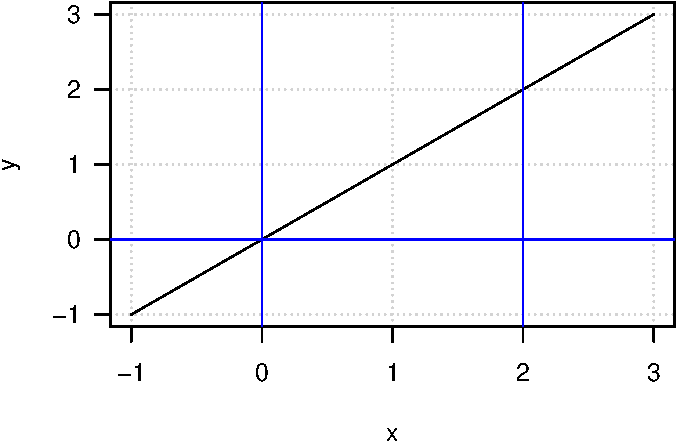
\includegraphics{105-math-integration_files/figure-latex/int-area-1} 

}

\caption{Graph of function $f(x) = x$}\label{fig:int-area}
\end{figure}

We write \[\int_{0}^2f(x)dx = \int_{0}^2 xdx =  \Bigr[ \frac{1}{2}x^2\Bigr]_0^2 = \frac{1}{2}(2)^2 - \frac{1}{2}(0)^2 = 2\] so first find the integral and then we evaluate it at upper limit and subtracting the evaluation at the lower limit. Here, the result it 2. What would be the result if you tried to calculate the triangle area on the above plot, area defined by the blue vertical lines drawn at 0 and 2 and horizontal x-axis? The formula for the triangle area is \(Area = \frac{1}{2}\cdot base \cdot height\) so here \(Area = \frac{1}{2} \cdot 2 \cdot 2 = 2\) the same result as achieved with integration.

\begin{center}\rule{0.5\linewidth}{0.5pt}\end{center}

\begin{exercise}
\protect\hypertarget{exr:m-int}{}{\label{exr:m-int} }
Integrate:

\begin{enumerate}
\def\labelenumi{\alph{enumi})}
\tightlist
\item
  \(\int 2 \cdot dx\)
\item
  \(\int 2x\cdot dx\)
\item
  \(\int (x^4 + x^2 + 1)\cdot dx\)
\item
  \(\int e^x\cdot dx\)
\item
  \(\int e^{2x}\cdot dx\)
\item
  \(\int \frac{2}{x}\cdot dx\)
\item
  \(\int_2^4 2x\cdot dx\)
\item
  \(\int_0^4 (x^2+1)dx\)
\item
  \(\int (x^4 + \frac{2}{x} + e^{2x}) dx\)
\item
  \(\int_0^4 (x^4+1) dx\)
\end{enumerate}
\end{exercise}

\hypertarget{answers-to-selected-exercises-integration}{%
\section*{Answers to selected exercises (integration)}\label{answers-to-selected-exercises-integration}}
\addcontentsline{toc}{section}{Answers to selected exercises (integration)}

Exr. \ref{exr:m-int}

\begin{enumerate}
\def\labelenumi{\alph{enumi})}
\tightlist
\item
  \(\int 2 \cdot dx = 2x +c\)
\item
  \(\int 2x\cdot dx = \frac{2x^2}{2} = x^2 + c\)
\item
  \(\int (x^4 + x^2 + 1)\cdot dx = \frac{x^5}{5} + \frac{x^3}{3} + x + c\)
\item
  \(\int e^x\cdot dx = e^x + c\)
\item
  \(\int e^{2x}\cdot dx = \frac{1}{2}e^{2x}\)
\item
  \(\int \frac{2}{x}\cdot dx =\int 2\cdot \frac{1}{x}\cdot dx = 2 \ln{x}+ c\)
\item
  \(\int_2^4 2x\cdot dx = \Bigr[x^2\Bigr]_2^4 = 16 - 4 = 12\)
\item
  \(\int_0^4 (x^2+1)dx = \Bigr[\frac{x^3}{3} + x \Bigr]_0^4=\frac{4^3}{3}+4 - 0 = \frac{64}{3}+4 = \frac{76}{3}\)
\end{enumerate}

\hypertarget{vectors}{%
\chapter{Vectors}\label{vectors}}

\textbf{Aims}

\begin{itemize}
\tightlist
\item
  to introduce vectors and basic vectors operations
\end{itemize}

\textbf{Learning outcomes}

\begin{itemize}
\tightlist
\item
  to be able to write \(n\)-dimensional vectors using vector notations
\item
  to be able to perform addition and scalar multiplication
\item
  to be able to check if two vectors are orthogonal
\end{itemize}

A large number of statistical models use vectors and matrices, both for compact representations, and for the calculations, e.g.~parameter estimates.

\hypertarget{vectors-1}{%
\section{Vectors}\label{vectors-1}}

\begin{itemize}
\tightlist
\item
  A vector is an ordered set of number
\item
  These numbers, e.g.~in vector \(\mathbf{x}\) can be expressed as a row \(\mathbf{x}=[6\quad 0\quad 5 \dots1]\)
\item
  or as a column \(\mathbf{x}=\begin{bmatrix} 6 \\ 0 \\ 5 \\ \vdots \\ 1 \end{bmatrix}\)
\item
  the number of elements in a vector is referred to as its \textbf{dimension} and we often use \(n\) to express \(n\)-dimensional vector, where \(n\) can be any natural number
\item
  here, we denote vectors using small bold font \(\mathbf{x}\), other notations may include an arrow \(\vec x\) or overline \(\overline{x}\)
\item
  also \textbf{parentheses} are used interchangeably with \textbf{square bracket}, e.g.~\(\mathbf{x}=[6\quad 0\quad 5 \dots1]\) can be written as \(\mathbf{x}=(6\quad 0\quad 5 \dots1)\) or \(\begin{pmatrix} 6\\ 0\\ 5\\ \vdots \\ 1 \end{pmatrix}\)
\end{itemize}

\hypertarget{operations-on-vectors}{%
\section{Operations on vectors}\label{operations-on-vectors}}

Given two vectors of the same dimension:
\(\mathbf{x}=\begin{bmatrix}  x_1 \\  x_2 \\  x_3 \\  \vdots \\  x_n \end{bmatrix}\)
and
\(\mathbf{y}=\begin{bmatrix}  y_1 \\  y_2 \\  y_3 \\  \vdots \\  y_n \end{bmatrix}\)

\textbf{Addition}: we add two vectors, element by element \(\mathbf{x} + \mathbf{y}=\begin{bmatrix}  x_1 + y_1 \\  x_2 + y_2 \\  x_3 + y_3 \\  \vdots \\  x_n + y_n \end{bmatrix}\)

\textbf{Scalar multiplication}: we can multiple vector by a numerical value, scalar, denoted as \(\gamma\):
\[\gamma \cdot \mathbf{x} =\begin{bmatrix}
  \gamma \cdot x_1 \\ 
  \gamma \cdot x_2 \\
  \gamma \cdot x_3 \\
  \vdots \\
  \gamma \cdot x_n 
\end{bmatrix}\]

\textbf{Difference} \(\mathbf{x} - \mathbf{y}\) can be written as \(\mathbf{x} + (-1) \cdot \mathbf{y}\), thus we multiply second vector with \(-1\) and then add two vectors

\textbf{Linear combination of vectors}: the vector \(\gamma \cdot \mathbf{x} + \delta \cdot \mathbf{y}\) is said to be a linear combination of \(\mathbf{x}\) and \(\mathbf{y}\):
\[\gamma \cdot \mathbf{x} + \delta \cdot \mathbf{y} =\begin{bmatrix}
  \gamma \cdot x_1 + \delta \cdot y_1 \\ 
  \gamma \cdot x_2 + \delta \cdot y_2\\
  \gamma \cdot x_3 + \delta \cdot y_3\\
  \vdots \\
  \gamma \cdot x_n + \delta \cdot y_n
\end{bmatrix}\]

\textbf{Inner product of vectors} is given by: \[\mathbf{x} \cdot \mathbf{y} = x_1 \cdot y_1 + x_2 \cdot y_2 + \dots x_n \cdot y_n = \displaystyle\sum_{i=1}^{n}x_i\cdot y_i\]

\textbf{Orthogonality of vectors}: two vectors are said to be orthogonal if their inner product is zero \[\mathbf{x} \cdot \mathbf{y} =\displaystyle\sum_{i=1}^{n}x_i\cdot y_i = 0\]

\hypertarget{null-and-unit-vector}{%
\section{Null and unit vector}\label{null-and-unit-vector}}

\begin{itemize}
\tightlist
\item
  a \textbf{null vector} is a vector whose elements are all \(0\); the difference between any vector and itself yields a null vector
\item
  a \textbf{unit vector} is a vector whose elements are all \(1\)
\end{itemize}

\begin{center}\rule{0.5\linewidth}{0.5pt}\end{center}

\begin{exercise}
\protect\hypertarget{exr:m-vectors}{}{\label{exr:m-vectors} }Based on vector definitions and operations:

\begin{enumerate}
\def\labelenumi{\alph{enumi})}
\item
  find the vector \(\mathbf{x} + \mathbf{y}\) when \(\mathbf{x} =\begin{bmatrix}  1 \\  2 \\  5 \end{bmatrix}\) and \(\mathbf{y} =\begin{bmatrix}  0\\  3 \\  1  \end{bmatrix}\)
\item
  find the vector \(2\mathbf{x} - \mathbf{y}\) when \(\mathbf{x} =\begin{bmatrix}  -2 \\  3 \\  5 \end{bmatrix}\) and \(\mathbf{y} =\begin{bmatrix}  0\\  -4 \\  7  \end{bmatrix}\)
\item
  are \(\mathbf{u}\) and \(\mathbf{v}\) vectors orthogonal when when \(\mathbf{u} =\begin{bmatrix}  1 \\  2 \end{bmatrix}\) and \(\mathbf{v} =\begin{bmatrix}  2\\  -1  \end{bmatrix}\)?
\item
  are \(\mathbf{u}\) and \(\mathbf{v}\) vectors orthogonal when when \(\mathbf{u} =\begin{bmatrix}  3 \\  -1 \end{bmatrix}\) and \(\mathbf{v} =\begin{bmatrix}  7\\  5  \end{bmatrix}\)?
\item
  find the value \(n\) such that the vectors \(\mathbf{u} =\begin{bmatrix}  2 \\  4 \\  1 \end{bmatrix}\) and \(\mathbf{v} =\begin{bmatrix}  n\\  1 \\  8  \end{bmatrix}\) are orthogonal.
\end{enumerate}
\end{exercise}

\hypertarget{answers-to-selected-exercises-vectors-and-matrices}{%
\section*{Answers to selected exercises (vectors and matrices)}\label{answers-to-selected-exercises-vectors-and-matrices}}
\addcontentsline{toc}{section}{Answers to selected exercises (vectors and matrices)}

Exr. \ref{exr:m-vectors}

\begin{enumerate}
\def\labelenumi{\alph{enumi})}
\tightlist
\item
\end{enumerate}

\[\mathbf{x} + \mathbf{y} = \begin{bmatrix} 1 \\ 2 \\ 5 \end{bmatrix} + \begin{bmatrix} 0 \\ 3 \\ 1 \end{bmatrix} = \begin{bmatrix} 1 + 0\\ 2 + 3 \\ 5 + 1 \end{bmatrix} = \begin{bmatrix} 1 \\ 5 \\ 6 \end{bmatrix}\]

\begin{enumerate}
\def\labelenumi{\alph{enumi})}
\setcounter{enumi}{1}
\item
  \[2\mathbf{x} - \mathbf{y} = \begin{bmatrix} 2 \cdot (-2) \\ 2 \cdot 3 \\ 2 \cdot 5 \end{bmatrix} + \begin{bmatrix} (-1) \cdot 0 \\ (-1) \cdot (-4) \\ (-1) \cdot 7 \end{bmatrix} = \begin{bmatrix} -4 \\ 6 \\ 10 \end{bmatrix}  + \begin{bmatrix} 0 \\ 4 \\ -7 \end{bmatrix}  = \begin{bmatrix} -4 + 0 \\ 6 + 4 \\ 10 - 7 \end{bmatrix} = \begin{bmatrix} -4 \\ 10 \\ 3 \end{bmatrix}\]
\item
  Yes, to check orthogonality we need to calculate the inner product of two vectors and see if it is equal to 0, here
  \(\mathbf{u} \cdot \mathbf{v} =\displaystyle\sum_{i=1}^{2}u_i\cdot v_i = 1 \cdot 2 + 2 \cdot (-1) = 2 - 2 = 0\)
\item
  No, since the inner product does not equal to 0 \[\mathbf{u} \cdot \mathbf{v} =\displaystyle\sum_{i=1}^{2}u_i\cdot v_i = 3 \cdot 7 + (-1) \cdot 5 = 21 - 5 = 16 \neq 0\]
\end{enumerate}

\hypertarget{matrices}{%
\chapter{Matrices}\label{matrices}}

\textbf{Aims}

\begin{itemize}
\tightlist
\item
  to introduce matrix and basic matrices operations
\end{itemize}

\textbf{Learning outcomes}

\begin{itemize}
\tightlist
\item
  to be able to write matrices using matrix notations
\item
  to be able to perform simple matrix operations such as adding and multiplication
\item
  to be able to find the reverse of the 2-dimensional matrix
\end{itemize}

\hypertarget{matrix}{%
\section{Matrix}\label{matrix}}

A matrix is a rectangular array of numbers e.g.~

\[\mathbf{A}=\begin{bmatrix}
  x_{11} & x_{12} & x_{13} & \dots & x_{1n} \\
  x_{21} & x_{22} & x_{23} & \dots & x_{2n} \\
  \dots & \dots & \dots& \dots & \dots\\
  x_{m1} & x_{m2} & x_{1m3} & \dots & x_{mn} \\
\end{bmatrix}\]

where:

\begin{itemize}
\tightlist
\item
  the notional subscripts in the typical element \(x_{ij}\) refers to its row and column location in the array, e.g.~\(x_{12}\) refers to element in the first row and second column
\item
  we say that matrix has \(m\) rows and \(n\) columns and the \textbf{dimension} of a matrix is defined as \(m \times n\)
\item
  a matrix can be viewed as a set of column vectors or a set of row vectors
\item
  a vector can be viewed as a matrix with only one column or with only one row
\end{itemize}

\hypertarget{special-matrices}{%
\section{Special matrices}\label{special-matrices}}

\begin{itemize}
\tightlist
\item
  A matrix with the same number of rows as columns, \(m = n\), is said to be a \textbf{square matrix}
\item
  A matrix that is not squared, \(m \neq n\) is called \textbf{rectangular matrix}
\item
  A \textbf{null matrix} is composed of all 0
\item
  An \textbf{identity matrix}, denoted as \(\mathbf{I}\) or \(\mathbf{I_n}\), is a square matrix with 1's on the main diagonal and all other elements equal to 0, e.g.~a three-dimensional identity matrix is \[\mathbf{I}=\begin{bmatrix}
  1 & 0 & 0  \\
  0 & 1 & 0  \\
  0 & 0 & 1
  \end{bmatrix}\]
\item
  A square matrix is said to be \textbf{symmetric} if \(x_{ij} = x_{ji}\) e.g.~
  \[\mathbf{A}=\begin{bmatrix}
  1 & 4 & 2  \\
  4 & 1 & 0  \\
  2 & 0 & 1
  \end{bmatrix}\]
\item
  A \textbf{diagonal matrix} is a square matrix whose non-diagonal entries are all zero, that is \(x_{ij} = 0\) for \(i \neq j\), e.g.~
  \[\mathbf{A}=\begin{bmatrix}
  1 & 0 & 0  \\
  0 & 2 & 0  \\
  0 & 0 & 3
  \end{bmatrix}\]
\item
  An \textbf{upper-triangular matrix} is a square matrix in which all entries below the diagonal are 0, that is \(x_{ij}=0\) for \(i<j\) e.g.~
  \[\mathbf{A}=\begin{bmatrix}
  1 & 3 & 4  \\
  0 & 2 & 5  \\
  0 & 0 & 3
  \end{bmatrix}\]
\item
  A \textbf{lower-triangular matrix} is a square matrix in which all entries above the digonal are 0, that is hat is \(x_{ij}=0\) for \(i>j\) e.g.~
  \[\mathbf{A}=\begin{bmatrix}
  1 & 0 & 0  \\
  1 & 1 & 0  \\
  1 & 1 & 1
  \end{bmatrix}\]
\end{itemize}

\hypertarget{matrix-operations}{%
\section{Matrix operations}\label{matrix-operations}}

\begin{itemize}
\tightlist
\item
  matrix \(\mathbf{A} = \mathbf{B}\) if both matrices have exactly the same dimension and if each element of \(\mathbf{A}\) equals to the corresponding element of e.g.~\(\mathbf{A} = \mathbf{B}\) if
  \(\mathbf{A}=\begin{bmatrix} 1 & 3 & 4 \\ 0 & 2 & 5 \\ 0 & 0 & 3 \end{bmatrix}\) and \(\mathbf{B}=\begin{bmatrix} 1 & 3 & 4 \\ 0 & 2 & 5 \\ 0 & 0 & 3 \end{bmatrix}\)
\end{itemize}

\begin{itemize}
\tightlist
\item
  for any matrix \(\mathbf{A}\) the \textbf{transpose}, denoted by \(\mathbf{A}^\top\) or \(\mathbf{A}^\prime\), is obtained by interchanging rows and columns, e.g.~given matrix \(\mathbf{A}=\begin{bmatrix} 1 & 3 & 4 \\ 0 & 2 & 5 \\ 0 & 0 & 3 \end{bmatrix}\) we have \(\mathbf{A}^\top=\begin{bmatrix} 1 & 0 & 0 \\ 3 & 2 & 0 \\ 4 & 5 & 3 \end{bmatrix}\). The transpose of a transpose of a matrix yield the original matrix, \(\Big(\mathbf{A}^\top\Big)^\top = \mathbf{A}\)
\end{itemize}

\begin{itemize}
\tightlist
\item
  we can \textbf{add} two matrices if they have the same dimension, e.g.~
  \[\mathbf{A} + \mathbf{B} = \mathbf{A} =\begin{bmatrix}
  x_{11} & x_{12}   \\
  x_{21} & x_{22} 
  \end{bmatrix} + \begin{bmatrix}
  y_{11} & y_{12}   \\
  y_{21} & y_{22} 
  \end{bmatrix} = \begin{bmatrix}
  x_{11}+y_{11} & x_{12}+y_{12}   \\
  x_{21}+y_{21} & x_{22}+y_{22} 
  \end{bmatrix}\]
\end{itemize}

\begin{itemize}
\tightlist
\item
  we can \textbf{multiply} a matrix by \textbf{a scalar} \(\delta\) e.g.~\[\delta \cdot \mathbf{A} = \begin{bmatrix}
  \delta \cdot x_{11} & \delta \cdot x_{12}   \\
  \delta \cdot x_{21} & \delta \cdot x_{22} 
  \end{bmatrix}\]
\end{itemize}

\begin{itemize}
\tightlist
\item
  we can \textbf{multiply two matrices} if they are \textbf{conformable}, i.e.~first matrix has the same number of columns as the number of rows in the second matrix. We then can write:
  \[\mathbf{C} = \mathbf{A} \cdot \mathbf{B}  = \begin{bmatrix}
  x_{11} & x_{12} & x_{13}  \\
  x_{21} & x_{22} & x_{23}
  \end{bmatrix} + \begin{bmatrix}
  y_{11} & y_{12}   \\
  y_{21} & y_{22}  \\
  y_{31} & y_{32}
  \end{bmatrix} = \\\ 
  \begin{bmatrix}
  x_{11} \cdot y_{11} + x_{12} \cdot y_{21} + x_{13} \cdot y_{31}  & x_{11} \cdot y_{12} + x_{12} \cdot y_{22} + x_{13} \cdot y_{32}  \\
  x_{21} \cdot y_{22} + x_{23} \cdot y_{21} + x_{13} \cdot y_{31} & x_{21} \cdot y_{12} + x_{23} \cdot y_{22} + x_{13} \cdot y_{32}
  \end{bmatrix}\]
\end{itemize}

\hypertarget{inverse-of-a-matrix}{%
\section{Inverse of a matrix}\label{inverse-of-a-matrix}}

For a square matrix \(\mathbf{A}\) there may exist a matrix \(\mathbf{B}\) such that \(\mathbf{A} \cdot \mathbf{B} = \mathbf{I}\). An \textbf{inverse}, if it exists, is denoted as \(\mathbf{A}^{-1}\) and we can rewrite the definition as \[\mathbf{A} \cdot \mathbf{A}^{-1} = \mathbf{I}\] where \(\mathbf{I}\) is an identify matrix (equivalent to 1). There is no division for matrices, instead we can use inverse to multiply the matrix by an inverse, similar to when instead of dividing the number \(a\) by \(b\) we multiply \(a\) by reciprocal of \(b = \frac{1}{b}\)

For a 2-dimensional matrix we can follow the below formula for obtaining the inverse
\[\begin{bmatrix}
  x_{11} & x_{12}   \\
  x_{21} & x_{22} 
\end{bmatrix}^{-1} = \frac{1}{x_{11} \cdot x_{22} - x_{12} \cdot x_{21}} \cdot \begin{bmatrix}
  x_{22} & -x_{12}   \\
  -x_{21} & x_{11} 
\end{bmatrix}\]

\hypertarget{orthogonal-matrix}{%
\section{Orthogonal matrix}\label{orthogonal-matrix}}

\begin{itemize}
\tightlist
\item
  A matrix \(\mathbf{A}\) for which \(\mathbf{A^\top} = \mathbf{A^{-1}}\) is true is said to be \textbf{orthogonal}
\end{itemize}

\begin{center}\rule{0.5\linewidth}{0.5pt}\end{center}

\begin{exercise}
\protect\hypertarget{exr:m-matrix}{}{\label{exr:m-matrix} }
Given matrices

\(\mathbf{A} = \begin{bmatrix}  1 & 2 \\  3 & 4  \end{bmatrix}\),
\(\mathbf{B} = \begin{bmatrix}  1 & 0 \\  0 & 1  \end{bmatrix}\) and \(\mathbf{C} = \begin{bmatrix}  1 & 0 \\  0 & 2  \end{bmatrix}\)

\begin{enumerate}
\def\labelenumi{\alph{enumi})}
\tightlist
\item
  what is the dimension of matrix \(\mathbf{A}\)?
\item
  what is \(\mathbf{A}^\top\)?
\item
  which of the matrices is i) an identity matrix ii) a square matrix, iii) null matrix, iv) diagonal matrix, v) a triangular matrix,?
\item
  calculate \(\mathbf{A} + \mathbf{B}\)?
\item
  calculate \(\mathbf{A} \cdot \mathbf{C}\)?
\item
  calculate \(\mathbf{B}^\top\)
\item
  calculate \(\mathbf{A}^{-1}\)
\item
  calculate \((\mathbf{A} + \mathbf{B})^{-1}\)
\end{enumerate}
\end{exercise}

\hypertarget{answers-to-selected-exercises-matrices}{%
\section*{Answers to selected exercises (matrices)}\label{answers-to-selected-exercises-matrices}}
\addcontentsline{toc}{section}{Answers to selected exercises (matrices)}

Exr. \ref{exr:m-matrix}

\begin{enumerate}
\def\labelenumi{\alph{enumi})}
\item
  \(2 \times 2\)
\item
  \(\mathbf{A}^\top = \begin{bmatrix}  1 & 3 \\  2 & 4  \end{bmatrix}\)
\item
  \begin{enumerate}
  \def\labelenumii{\roman{enumii})}
  \tightlist
  \item
    identity matrix: \(\mathbf{B}\), ii) a square matrix: \(\mathbf{A}\), \(\mathbf{B}\) and \(\mathbf{C}\), iii) null matrix: none, iv) diagonal matrix: \(\mathbf{B}\) (identity matrix is diagonal) and \(\mathbf{C}\), v) triangular \(\mathbf{B}\) and \(\mathbf{C}\) as both identify matrix \(\mathbf{B}\) and diagonal matrix \(\mathbf{C}\) is triangular, both lower and upper triangular
  \end{enumerate}
\item
  \(\mathbf{A} + \mathbf{B} = \begin{bmatrix}  1 & 2 \\  3 & 4  \end{bmatrix} + \begin{bmatrix}  1 & 0 \\  0 & 1  \end{bmatrix} = \begin{bmatrix}  2 & 2 \\  3 & 5  \end{bmatrix}\)
\item
  \(\mathbf{A} \cdot \mathbf{C} = \begin{bmatrix}  1 \cdot 1 + 2 \cdot 0 & 1 \cdot 0 + 2 \cdot 2 \\  3 \cdot 1 + 4 \cdot 0 & 3 \cdot 0 + 4 \cdot 2  \end{bmatrix} = \begin{bmatrix}  1 & 4 \\  3 & 8  \end{bmatrix}\)
\item
  \(\mathbf{B}^\top = \begin{bmatrix}  1 & 0 \\  0 & 1  \end{bmatrix}\)
\item
\end{enumerate}

\[\mathbf{A}^{-1} = \begin{bmatrix}
  1 & 2   \\
  3 & 4 
\end{bmatrix}^{-1} = \frac{1}{1 \cdot 4 - 2 \cdot 3} \cdot \begin{bmatrix}
  4 & -2   \\
  -3 & 1
\end{bmatrix} = -\frac{1}{2} \cdot \begin{bmatrix}
  4 & -2   \\
  -3 & 1
\end{bmatrix} = \begin{bmatrix}
  -2 & 1   \\
  \frac{3}{2} & -\frac{1}{2}
\end{bmatrix}\]

\hypertarget{part-linear-models}{%
\part{Linear Models}\label{part-linear-models}}

\hypertarget{introduction-to-linear-models}{%
\chapter{Introduction to linear models}\label{introduction-to-linear-models}}

\textbf{Aims}

\begin{itemize}
\tightlist
\item
  to introduce concept of linear models using simple linear regression
\end{itemize}

\textbf{Learning outcomes}

\begin{itemize}
\tightlist
\item
  to understand what a linear model is and be familiar with the terminology
\item
  to be able to state linear model in the general vector-matrix notation
\item
  to be able to use the general vector-matrix notation to numerically estimate model parameters
\item
  to be able to use \texttt{lm()} function for model fitting, parameter estimation, hypothesis testing and prediction
\end{itemize}

\hypertarget{statistical-vs.-deterministic-relationship}{%
\section{Statistical vs.~deterministic relationship}\label{statistical-vs.-deterministic-relationship}}

Relationships in probability and statistics can generally be one of three things: deterministic, random, or statistical:

\begin{itemize}
\tightlist
\item
  a \textbf{deterministic} relationship involves \textbf{an exact relationship} between two variables, for instance Fahrenheit and Celsius degrees is defined by an equation \(Fahrenheit=\frac{9}{5}\cdot Celcius+32\)
\item
  there is \textbf{no relationship} between variables in the \textbf{random relationship}, for instance number of succulents Olga buys and time of the year as Olga keeps buying succulents whenever she feels like it throughout the entire year
\item
  \textbf{a statistical relationship} is a \textbf{mixture of deterministic and random relationship}, e.g.~the savings that Olga has left in the bank account depend on Olga's monthly salary income (deterministic part) and the money spent on buying succulents (random part)
\end{itemize}

\begin{figure}

{\centering 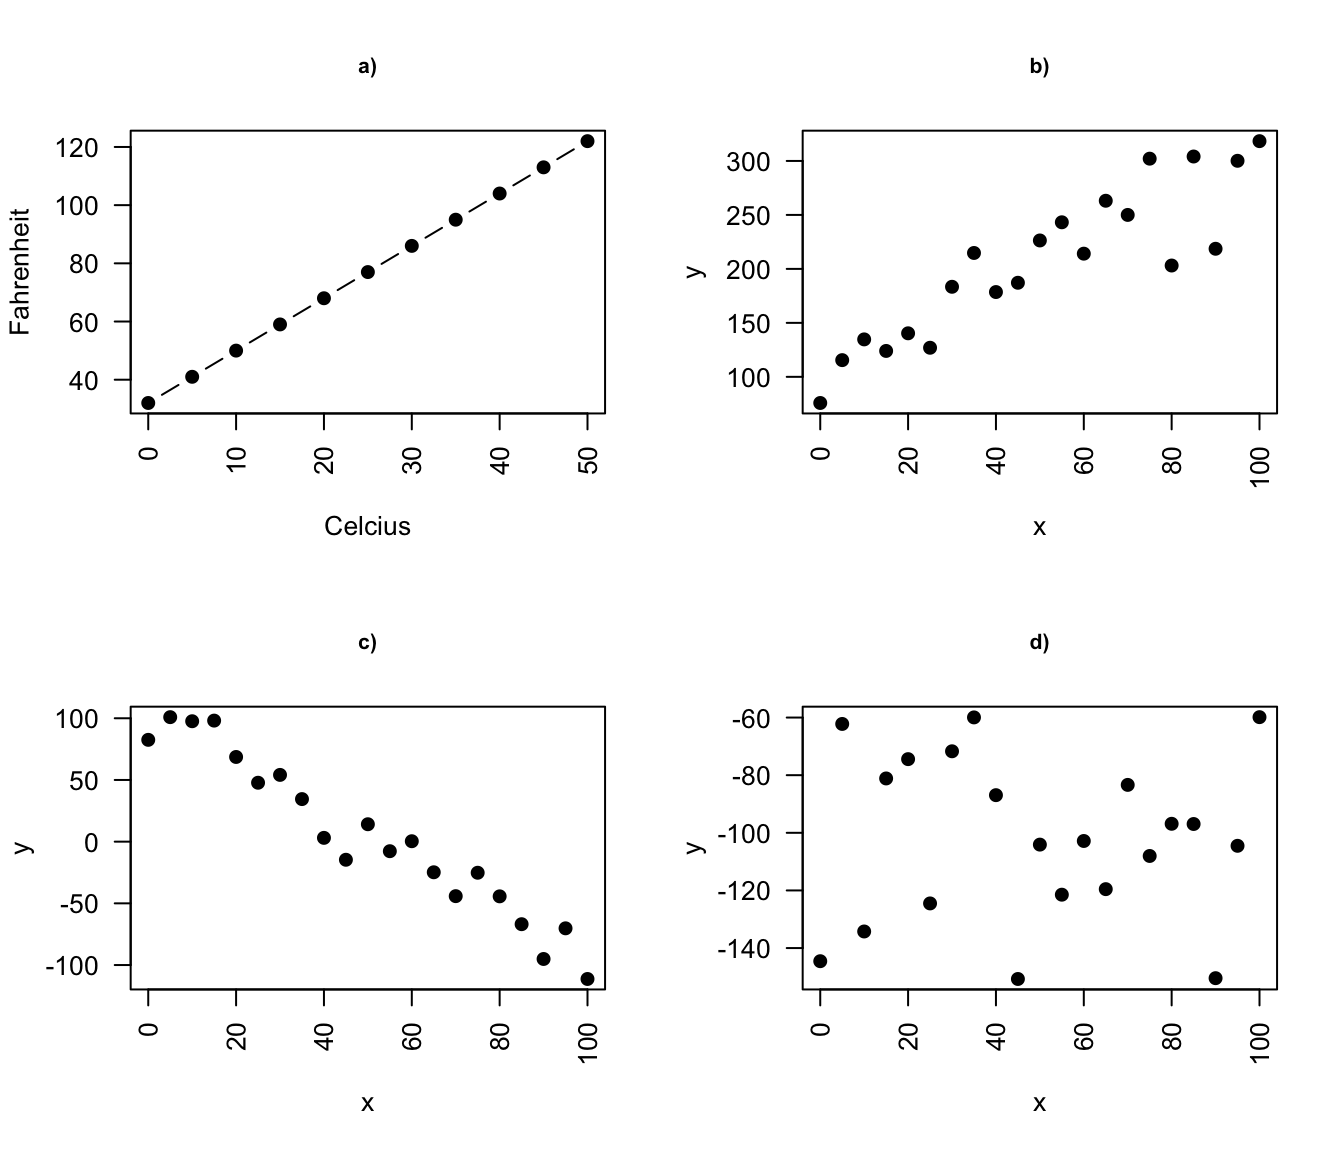
\includegraphics{301-linear-models_files/figure-latex/regression-deterministic-1} 

}

\caption{Deterministic vs. statistical relationship: a) deterministic: equation exactly describes the relationship between the two variables e.g. Ferenheit and Celcius relationship ; b) statistical relationship between $x$ and $y$ is not perfect (increasing relationship), c)  statistical relationship between $x$ and $y$ is not perfect (decreasing relationship), d) random signal}\label{fig:regression-deterministic}
\end{figure}

\hypertarget{what-linear-models-are-and-are-not}{%
\section{What linear models are and are not}\label{what-linear-models-are-and-are-not}}

\begin{itemize}
\tightlist
\item
  A linear model is one in which the parameters appear linearly in the deterministic part of the model
\item
  e.g.~\textbf{simple linear regression} through the origin is a simple linear model of the form \(Y_i = \beta x + \epsilon\) often used to express a relationship of one numerical variable to another, e.g.~the calories burnt and the kilometers cycled
\item
  linear models can become quite advanced by including more variables, e.g.~the calories burnt could be a function of both the kilometers cycled and status of bike, or the transformation of the variables
\end{itemize}

More examples where model parameters appear linearly:

\begin{itemize}
\tightlist
\item
  \(Y_i = \alpha + \beta x_i + \gamma x_i + \epsilon_i\)
\item
  \(Y_i = \alpha + \beta x_i^2 \epsilon\)
\item
  \(Y_i = \alpha + \beta x_i^2 + \gamma x_i^3 + \epsilon\)
\end{itemize}

and an example on a non-linear model where parameter \(\beta\) appears in the exponent of \(x_i\)

\begin{itemize}
\tightlist
\item
  \(Y_i = \alpha + x_i^\beta + \epsilon\)
\end{itemize}

\hypertarget{terminology}{%
\section{Terminology}\label{terminology}}

There are many terms and notations used interchangeably:

\begin{itemize}
\tightlist
\item
  \(y\) is being called:

  \begin{itemize}
  \tightlist
  \item
    response
  \item
    outcome
  \item
    dependent variable
  \end{itemize}
\item
  \(x\) is being called:

  \begin{itemize}
  \tightlist
  \item
    exposure
  \item
    explanatory variable
  \item
    dependent variable
  \item
    predictor
  \item
    covariate
  \end{itemize}
\end{itemize}

\hypertarget{with-linear-models-we-can-answer-questions-such-as}{%
\section{With linear models we can answer questions such as:}\label{with-linear-models-we-can-answer-questions-such-as}}

\begin{itemize}
\tightlist
\item
  is there a relationship between exposure and outcome, e.g.~body weight and plasma volume?
\item
  how strong is the relationship between the two variables?
\item
  what will be a predicted value of the outcome given a new set of exposure values?
\item
  how accurately can we predict outcome?
\item
  which variables are associated with the response, e.g.~is it body weight and height that can explain the plasma volume or is it just the body weight?
\end{itemize}

\hypertarget{simple-linear-regression}{%
\section{Simple linear regression}\label{simple-linear-regression}}

\begin{itemize}
\tightlist
\item
  It is used to check the association between the numerical outcome and one numerical explanatory variable
\item
  In practice, we are finding the best-fitting straight line to describe the relationship between the outcome and exposure
\item
  For example, let's look at the example data containing body weight (kg) and plasma volume (liters) for eight healthy men to see what the best-fitting straight line is.
\end{itemize}

Example data:

\begin{Shaded}
\begin{Highlighting}[]
\NormalTok{weight \textless{}{-}}\StringTok{ }\KeywordTok{c}\NormalTok{(}\DecValTok{58}\NormalTok{, }\DecValTok{70}\NormalTok{, }\DecValTok{74}\NormalTok{, }\FloatTok{63.5}\NormalTok{, }\FloatTok{62.0}\NormalTok{, }\FloatTok{70.5}\NormalTok{, }\FloatTok{71.0}\NormalTok{, }\FloatTok{66.0}\NormalTok{) }\CommentTok{\# body weight (kg)}
\NormalTok{plasma \textless{}{-}}\StringTok{ }\KeywordTok{c}\NormalTok{(}\FloatTok{2.75}\NormalTok{, }\FloatTok{2.86}\NormalTok{, }\FloatTok{3.37}\NormalTok{, }\FloatTok{2.76}\NormalTok{, }\FloatTok{2.62}\NormalTok{, }\FloatTok{3.49}\NormalTok{, }\FloatTok{3.05}\NormalTok{, }\FloatTok{3.12}\NormalTok{) }\CommentTok{\# plasma volume (liters)}
\end{Highlighting}
\end{Shaded}

\begin{figure}

{\centering 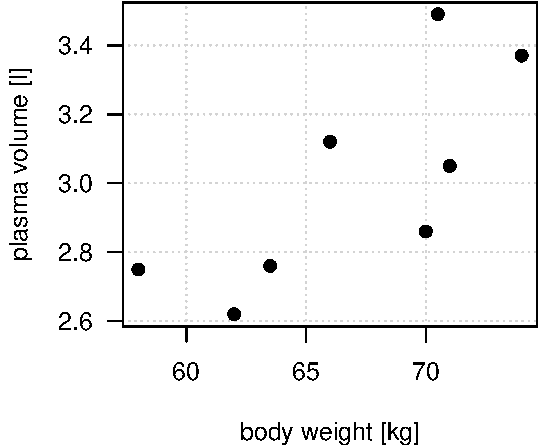
\includegraphics{301-linear-models_files/figure-latex/fig-intro-example-1} 

}

\caption{Scatter plot of the data shows that high plasma volume tends to be associated with high weight and *vice verca*.}\label{fig:fig-intro-example}
\end{figure}

\begin{figure}

{\centering 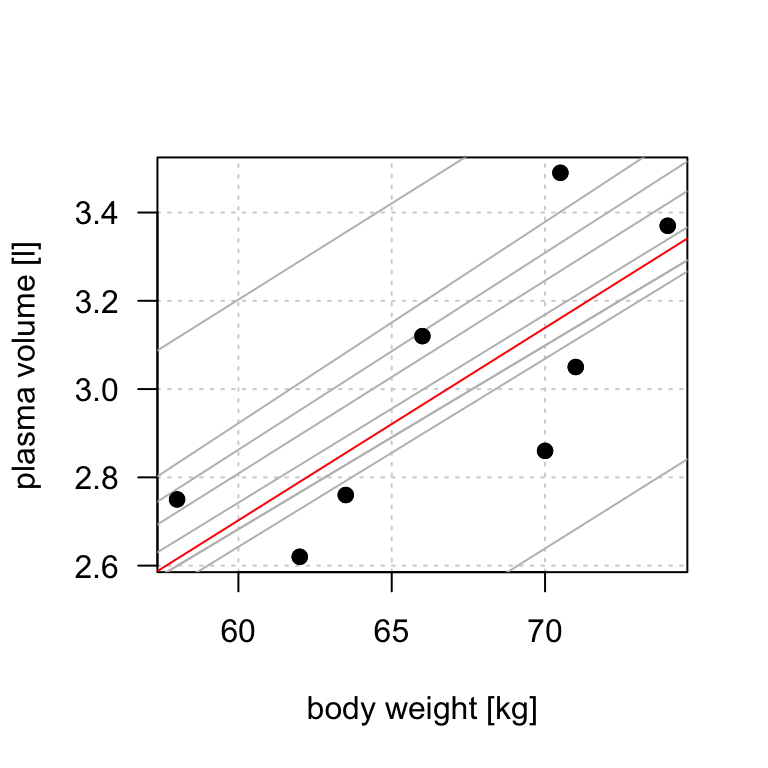
\includegraphics{301-linear-models_files/figure-latex/fig-intro-example-reg-1} 

}

\caption{Scatter plot of the data shows that high plasma volume tends to be associated with high weight and *vice verca*. Linear regression gives the equation of the straight line (red) that best describes how the outcome changes (increase or decreases) with a change of exposure variable}\label{fig:fig-intro-example-reg}
\end{figure}

The equation for the red line is:
\[Y_i=0.086 +  0.044 \cdot x_i \quad for \;i = 1 \dots 8\]
and in general:
\[Y_i=\alpha + \beta \cdot x_i \quad for \; i = 1 \dots n\]

\begin{itemize}
\tightlist
\item
  In other words, by finding the best-fitting straight line we are \textbf{building a statistical model} to represent the relationship between plasma volume (\(Y\)) and explanatory body weight variable (\(x\))
\item
  If were to use our model \(Y_i=0.086 + 0.044 \cdot x_i\) to find plasma volume given a weight of 58 kg (our first observation, \(i=1\)), we would notice that we would get \(Y=0.086 + 0.044 \cdot 58 = 2.638\), not exactly \(2.75\) as we have for our first man in our dataset that we started with, i.e.~\(2.75 - 2.638 = 0.112 \neq 0\).
\item
  We thus add to the above equation an \textbf{error term} to account for this and now we can write our \textbf{simple regression model} more formally as:
\end{itemize}

\begin{equation}
Y_i=\alpha + \beta \cdot x_i + \epsilon_i
\label{eq:regression-linear}
\end{equation}

where:

\begin{itemize}
\tightlist
\item
  we call \(\alpha\) and \(\beta\) \textbf{model coefficients}
\item
  and \(\epsilon_i\) \textbf{error terms}
\end{itemize}

\hypertarget{least-squares}{%
\section{Least squares}\label{least-squares}}

\begin{itemize}
\tightlist
\item
  in the above body weight - plasma volume example, the values of \(\alpha\) and \(\beta\) have just appeared
\item
  in practice, \(\alpha\) and \(\beta\) values are unknown and we use data to \textbf{estimate these coefficients}, noting the estimates with a \textbf{hat}, \(\hat{\alpha}\) and \(\hat{\beta}\)
\item
  \textbf{least squares} is one of the methods of parameters estimation, i.e.~finding \(\hat{\alpha}\) and \(\hat{\beta}\)
\end{itemize}

\begin{figure}

{\centering 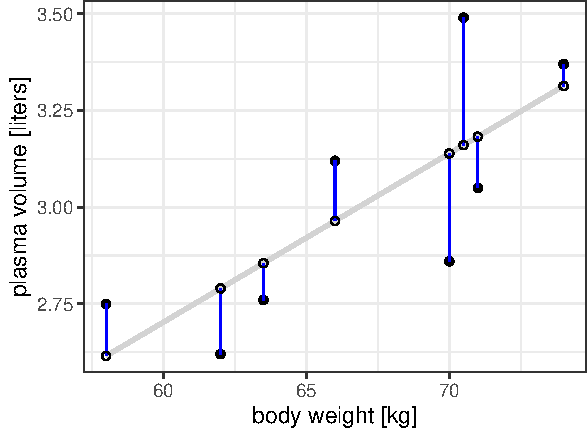
\includegraphics{301-linear-models_files/figure-latex/regression-errors-1} 

}

\caption{Scatter plot of the data shows that high plasma volume tends to be associated with high weight and *vice verca*. Linear regrssion gives the equation of the straight line (red) that best describes how the outcome changes with a change of exposure variable. Blue lines represent error terms, the vertical distances to the regression line}\label{fig:regression-errors}
\end{figure}

~\\
Let \(\hat{y_i}=\hat{\alpha} + \hat{\beta}x_i\) be the prediction \(y_i\) based on the \(i\)-th value of \(x\):

\begin{itemize}
\tightlist
\item
  Then \(\epsilon_i = y_i - \hat{y_i}\) represents the \(i\)-th \textbf{residual}, i.e.~the difference between the \(i\)-th observed response value and the \(i\)-th response value that is predicted by the linear model
\item
  RSS, the \textbf{residual sum of squares} is defined as: \[RSS = \epsilon_1^2 + \epsilon_2^2 + \dots + \epsilon_n^2\] or
  equivalently as: \[RSS=(y_1-\hat{\alpha}-\hat{\beta}x_1)^2+(y_2-\hat{\alpha}-\hat{\beta}x_2)^2+...+(y_n-\hat{\alpha}-\hat{\beta}x_n)^2\]
\item
  the least squares approach chooses \(\hat{\alpha}\) and \(\hat{\beta}\) \textbf{to minimize the RSS}. With some calculus we get Theorem \ref{thm:leastsq-01}
\end{itemize}

~\\
\begin{theorem}[Least squares estimates for a simple linear regression]
\protect\hypertarget{thm:leastsq-01}{}{\label{thm:leastsq-01} \iffalse (Least squares estimates for a simple linear regression) \fi{} }
\[\hat{\beta} = \frac{S_{xy}}{S_{xx}}\]
\[\hat{\alpha} = \bar{y}-\frac{S_{xy}}{S_{xx}}\cdot \bar{x}\]

where:

\begin{itemize}
\tightlist
\item
  \(\bar{x}\): mean value of \(x\)
\item
  \(\bar{y}\): mean value of \(y\)
\item
  \(S_{xx}\): sum of squares of \(X\) defined as \(S_{xx} = \displaystyle \sum_{i=1}^{n}(x_i-\bar{x})^2\)
\item
  \(S_{yy}\): sum of squares of \(Y\) defined as \(S_{yy} = \displaystyle \sum_{i=1}^{n}(y_i-\bar{y})^2\)
\item
  \(S_{xy}\): sum of products of \(X\) and \(Y\) defined as \(S_{xy} = \displaystyle \sum_{i=1}^{n}(x_i-\bar{x})(y_i-\bar{y})\)
\end{itemize}
\end{theorem}

We can further re-write the above sum of squares to obtain

\begin{itemize}
\tightlist
\item
  sum of squares of \(X\), \[S_{xx} = \displaystyle \sum_{i=1}^{n}(x_i-\bar{x})^2 = \sum_{i=1}^{n}x_i^2-\frac{(\sum_{i=1}^{n}x_i)^2}{n})\]
\item
  sum of products of \(X\) and \(Y\)
\end{itemize}

\[S_{xy} = \displaystyle \sum_{i=1}^{n}(x_i-\bar{x})(y_i-\bar{y})=\sum_{i=1}^nx_iy_i-\frac{\sum_{i=1}^{n}x_i\sum_{i=1}^{n}y_i}{n}\]

\textbf{Example (Least squares)}

Let's try least squares method to find coefficient estimates in our body weight and plasma volume example

\begin{Shaded}
\begin{Highlighting}[]
\CommentTok{\# initial data}
\NormalTok{weight \textless{}{-}}\StringTok{ }\KeywordTok{c}\NormalTok{(}\DecValTok{58}\NormalTok{, }\DecValTok{70}\NormalTok{, }\DecValTok{74}\NormalTok{, }\FloatTok{63.5}\NormalTok{, }\FloatTok{62.0}\NormalTok{, }\FloatTok{70.5}\NormalTok{, }\FloatTok{71.0}\NormalTok{, }\FloatTok{66.0}\NormalTok{) }\CommentTok{\# body weight (kg)}
\NormalTok{plasma \textless{}{-}}\StringTok{ }\KeywordTok{c}\NormalTok{(}\FloatTok{2.75}\NormalTok{, }\FloatTok{2.86}\NormalTok{, }\FloatTok{3.37}\NormalTok{, }\FloatTok{2.76}\NormalTok{, }\FloatTok{2.62}\NormalTok{, }\FloatTok{3.49}\NormalTok{, }\FloatTok{3.05}\NormalTok{, }\FloatTok{3.12}\NormalTok{) }\CommentTok{\# plasma volume (liters)}

\CommentTok{\# rename variables for convenience}
\NormalTok{x \textless{}{-}}\StringTok{ }\NormalTok{weight}
\NormalTok{y \textless{}{-}}\StringTok{ }\NormalTok{plasma}

\CommentTok{\# mean values of x and y}
\NormalTok{x.bar \textless{}{-}}\StringTok{ }\KeywordTok{mean}\NormalTok{(x)}
\NormalTok{y.bar \textless{}{-}}\StringTok{ }\KeywordTok{mean}\NormalTok{(y)}

\CommentTok{\# Sum of squares}
\NormalTok{Sxx \textless{}{-}}\StringTok{  }\KeywordTok{sum}\NormalTok{((x }\OperatorTok{{-}}\StringTok{ }\NormalTok{x.bar)}\OperatorTok{\^{}}\DecValTok{2}\NormalTok{)}
\NormalTok{Sxy \textless{}{-}}\StringTok{ }\KeywordTok{sum}\NormalTok{((x}\OperatorTok{{-}}\NormalTok{x.bar)}\OperatorTok{*}\NormalTok{(y}\OperatorTok{{-}}\NormalTok{y.bar))}

\CommentTok{\# Coefficient estimates}
\NormalTok{beta.hat \textless{}{-}}\StringTok{ }\NormalTok{Sxy }\OperatorTok{/}\StringTok{ }\NormalTok{Sxx}
\NormalTok{alpha.hat \textless{}{-}}\StringTok{ }\NormalTok{y.bar }\OperatorTok{{-}}\StringTok{ }\NormalTok{Sxy}\OperatorTok{/}\NormalTok{Sxx}\OperatorTok{*}\NormalTok{x.bar}

\CommentTok{\# Print estimated coefficients alpha and beta}
\KeywordTok{print}\NormalTok{(alpha.hat)}
\CommentTok{\#\# [1] 0.08572428}

\KeywordTok{print}\NormalTok{(beta.hat)}
\CommentTok{\#\# [1] 0.04361534}
\end{Highlighting}
\end{Shaded}

In R we can use \texttt{lm}, the built-in function, to fit a linear regression model and we can replace the above code with one line

\begin{Shaded}
\begin{Highlighting}[]
\KeywordTok{lm}\NormalTok{(plasma }\OperatorTok{\textasciitilde{}}\StringTok{ }\NormalTok{weight)}
\CommentTok{\#\# }
\CommentTok{\#\# Call:}
\CommentTok{\#\# lm(formula = plasma \textasciitilde{} weight)}
\CommentTok{\#\# }
\CommentTok{\#\# Coefficients:}
\CommentTok{\#\# (Intercept)       weight  }
\CommentTok{\#\#     0.08572      0.04362}
\end{Highlighting}
\end{Shaded}

\hypertarget{intercept-and-slope}{%
\section{Intercept and Slope}\label{intercept-and-slope}}

\begin{itemize}
\tightlist
\item
  Linear regression gives us estimates of model coefficient \(Y_i = \alpha + \beta x_i + \epsilon_i\)
\item
  \(\alpha\) is known as the \textbf{intercept}
\item
  \(\beta\) is known as the \textbf{slope}
\end{itemize}

\begin{figure}

{\centering 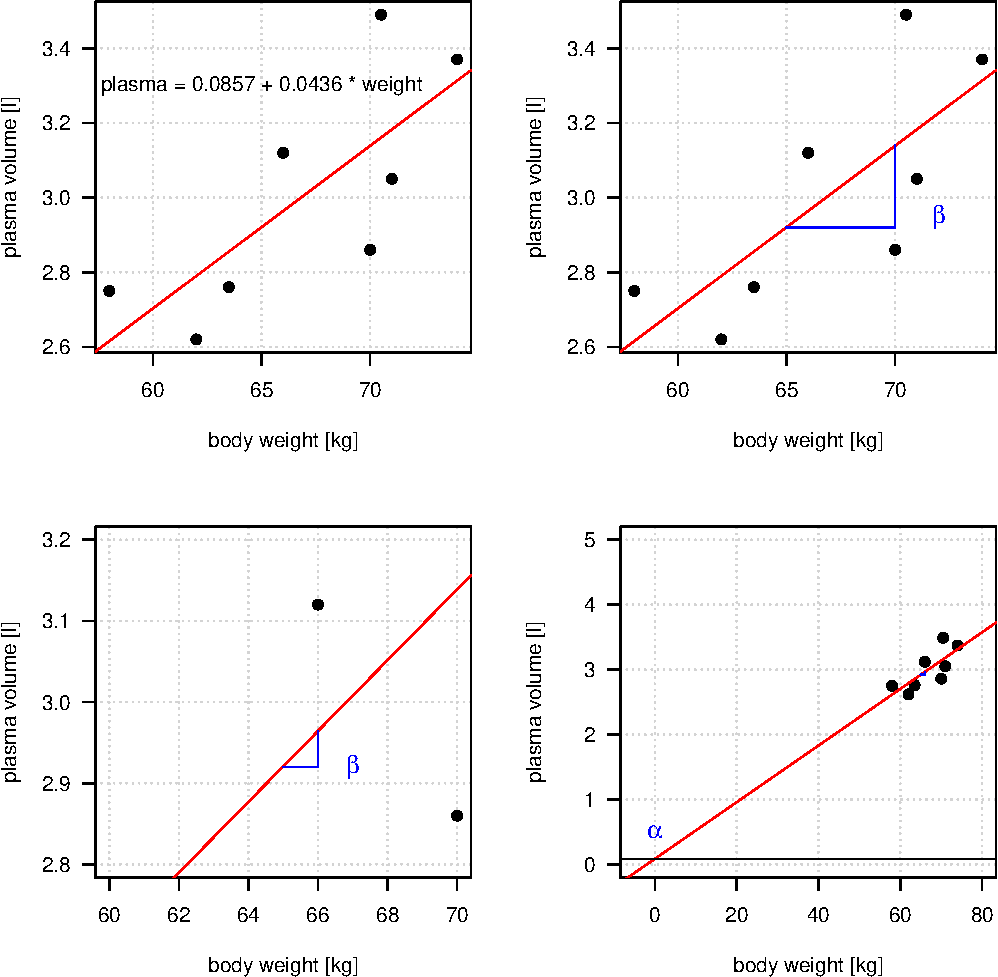
\includegraphics{301-linear-models_files/figure-latex/lm-parameters-1} 

}

\caption{Scatter plot of the data shows that high plasma volume tends to be associated with high weight and *vice verca*. Linear regression gives the equation of the straight line that best describes how the outcome changes (increase or decreases) with a change of exposure variable (in red)}\label{fig:lm-parameters}
\end{figure}

\hypertarget{hypothesis-testing}{%
\section{Hypothesis testing}\label{hypothesis-testing}}

\begin{itemize}
\tightlist
\item
  the calculated \(\hat{\alpha}\) and \(\hat{\beta}\) are estimates of the population values of the intercept and slope and are therefore subject to \textbf{sampling variation}
\item
  their precision is measure by their ** estimated standard errors**, e.s.e(\(\hat{\alpha}\)) and e.s.e(\(\hat{\beta}\))
\item
  these estimated standard errors are used in hypothesis testing and building confidence and prediction intervals
\end{itemize}

The most common hypothesis test involves testing the \texttt{null\ hypothesis} of:

\begin{itemize}
\tightlist
\item
  \(H_0:\) There is no relationship between \(X\) and \(Y\)
\item
  versus the \texttt{alternative\ hypothesis} \(H_a:\) there is some relationship between \(X\) and \(Y\)
\end{itemize}

Mathematically, this corresponds to testing:

\begin{itemize}
\tightlist
\item
  \(H_0: \beta=0\)
\item
  versus \(H_0: \beta\neq0\)
\item
  since if \(\beta=0\) then the model \(Y_i=\alpha+\beta x_i + \epsilon_i\) reduces to \(Y=\alpha + \epsilon_i\)
\end{itemize}

Under the null hypothesis:

\begin{itemize}
\tightlist
\item
  \(H_0: \beta = 0\) we have: \(\frac{\hat{\beta}-\beta}{e.s.e(\hat{\beta})} \sim t(n-p)\), where
\item
  \(n\) is number of observations
\item
  \(p\) is number of model parameters
\item
  \(\frac{\hat{\beta}-\beta}{e.s.e(\hat{\beta})}\) is called the t-statistics
\item
  that follows Student's t distribution with \(n-p\) degrees of freedom
\end{itemize}

\textbf{Example (Hypothesis testing)}

Let's look again at our example data. This time we will not only fit the linear regression model but look a bit more closely at the R summary of the model

\begin{Shaded}
\begin{Highlighting}[]
\NormalTok{weight \textless{}{-}}\StringTok{ }\KeywordTok{c}\NormalTok{(}\DecValTok{58}\NormalTok{, }\DecValTok{70}\NormalTok{, }\DecValTok{74}\NormalTok{, }\FloatTok{63.5}\NormalTok{, }\FloatTok{62.0}\NormalTok{, }\FloatTok{70.5}\NormalTok{, }\FloatTok{71.0}\NormalTok{, }\FloatTok{66.0}\NormalTok{) }\CommentTok{\# body weight (kg)}
\NormalTok{plasma \textless{}{-}}\StringTok{ }\KeywordTok{c}\NormalTok{(}\FloatTok{2.75}\NormalTok{, }\FloatTok{2.86}\NormalTok{, }\FloatTok{3.37}\NormalTok{, }\FloatTok{2.76}\NormalTok{, }\FloatTok{2.62}\NormalTok{, }\FloatTok{3.49}\NormalTok{, }\FloatTok{3.05}\NormalTok{, }\FloatTok{3.12}\NormalTok{) }\CommentTok{\# plasma volume (liters)}

\NormalTok{model \textless{}{-}}\StringTok{ }\KeywordTok{lm}\NormalTok{(plasma }\OperatorTok{\textasciitilde{}}\StringTok{ }\NormalTok{weight)}
\KeywordTok{print}\NormalTok{(}\KeywordTok{summary}\NormalTok{(model))}
\CommentTok{\#\# }
\CommentTok{\#\# Call:}
\CommentTok{\#\# lm(formula = plasma \textasciitilde{} weight)}
\CommentTok{\#\# }
\CommentTok{\#\# Residuals:}
\CommentTok{\#\#      Min       1Q   Median       3Q      Max }
\CommentTok{\#\# {-}0.27880 {-}0.14178 {-}0.01928  0.13986  0.32939 }
\CommentTok{\#\# }
\CommentTok{\#\# Coefficients:}
\CommentTok{\#\#             Estimate Std. Error t value Pr(\textgreater{}|t|)  }
\CommentTok{\#\# (Intercept)  0.08572    1.02400   0.084   0.9360  }
\CommentTok{\#\# weight       0.04362    0.01527   2.857   0.0289 *}
\CommentTok{\#\# {-}{-}{-}}
\CommentTok{\#\# Signif. codes:  0 \textquotesingle{}***\textquotesingle{} 0.001 \textquotesingle{}**\textquotesingle{} 0.01 \textquotesingle{}*\textquotesingle{} 0.05 \textquotesingle{}.\textquotesingle{} 0.1 \textquotesingle{} \textquotesingle{} 1}
\CommentTok{\#\# }
\CommentTok{\#\# Residual standard error: 0.2188 on 6 degrees of freedom}
\CommentTok{\#\# Multiple R{-}squared:  0.5763,	Adjusted R{-}squared:  0.5057 }
\CommentTok{\#\# F{-}statistic:  8.16 on 1 and 6 DF,  p{-}value: 0.02893}
\end{Highlighting}
\end{Shaded}

\begin{itemize}
\tightlist
\item
  Under ``Estimate'' we see estimates of our model coefficients, \(\hat{\alpha}\) (intercept) and \(\hat{\beta}\) (slope, here weight), followed by their estimated standard errors.
\item
  If we were to test if there is an association between weight and plasma volume we would write under \(H_0: \beta = 0\) and \(\frac{\hat{\beta}-\beta}{e.s.e(\hat{\beta})} = \frac{0.04362-0}{0.01527} = 2.856582\)
\item
  and we would compare t-statistics to Student's t distribution with \(n-p = 8 - 2 = 6\) degrees of freedom (we have two model parameters, \(\alpha\) and \(\beta\))
\item
  we can use Student's t distribution table or R code to obtain the p-value
\end{itemize}

\begin{Shaded}
\begin{Highlighting}[]
\DecValTok{2}\OperatorTok{*}\KeywordTok{pt}\NormalTok{(}\FloatTok{2.856582}\NormalTok{, }\DataTypeTok{df=}\DecValTok{6}\NormalTok{, }\DataTypeTok{lower=}\NormalTok{F)}
\CommentTok{\#\# [1] 0.02893095}
\end{Highlighting}
\end{Shaded}

\begin{itemize}
\tightlist
\item
  here the observed t-statistics is large and therefore yields a small p-value, meaning that there is sufficient evidence to reject null hypothesis in favor of the alternative and conclude that there is an significant association between weight and plasma volume
\end{itemize}

\hypertarget{vector-matrix-notations}{%
\section{Vector-matrix notations}\label{vector-matrix-notations}}

While in simple linear regression it is feasible to arrive at the parameters estimates using calculus in more realistic settings with multiple regression (more than one explanatory variable in the model) it is more efficient to use vectors and matrices to define the regression model.

Let's rewrite our simple linear regression model \(Y_i = \alpha + \beta_i + \epsilon_i \quad i=1,\dots n\) into vector-matrix notations.

\begin{itemize}
\tightlist
\item
  First we rename our \(\alpha\) to \(\beta_0\) and \(\beta\) to \(\beta_1\) (it is easier to keep tracking the number of model parameters this way)
\item
  Then we notice that we actually have \(n\) equations such as:
  \[y_1 = \beta_0 + \beta_1 x_1 + \epsilon_1\]
  \[y_2 = \beta_0 + \beta_1 x_2 + \epsilon_2\]
  \[y_3 = \beta_0 + \beta_1 x_3 + \epsilon_3\]
  \[\dots\]
  \[y_n = \beta_0 + \beta_1 x_n + \epsilon_n\]
\item
  we can group all \(Y_i\) and \(\epsilon_i\) into column vectors:
  \(\mathbf{Y}=\begin{bmatrix} y_1 \\ y_2 \\ \vdots \\ y_{n} \end{bmatrix}\) and
  \(\boldsymbol\epsilon=\begin{bmatrix} \epsilon_1 \\ \epsilon_2 \\ \vdots \\ \epsilon_{n} \end{bmatrix}\)
\item
  we stack two parameters \(\beta_0\) and \(\beta_1\) into another column vector:\[\boldsymbol\beta=\begin{bmatrix}
  \beta_0  \\
  \beta_1
  \end{bmatrix}\]
\item
  we then append a vector of ones with the single predictor for each \(i\) and create a matrix with two columns:
  design matrix \[\mathbf{X}=\begin{bmatrix}
  1 & x_1  \\
  1 & x_2  \\
  \vdots & \vdots \\
  1 & x_{n}
  \end{bmatrix}\]
\end{itemize}

Now we can write our linear model in a vector-matrix notations as:
\[\mathbf{Y} = \boldsymbol\beta\mathbf{X} + \boldsymbol\epsilon\]

\textbf{Definition: vector matrix form of the linear model}

The vector-matrix representation of a linear model with \(p-1\) predictors can be written as
\[\mathbf{Y} = \boldsymbol\beta\mathbf{X} + \boldsymbol\epsilon\]

where:

\begin{itemize}
\tightlist
\item
  \(\mathbf{Y}\) is \(n \times1\) vector of observations
\item
  \(\boldsymbol\beta\) is \(p \times1\) vector of parameters
\item
  \(\mathbf{X}\) is \(n \times p\) design matrix
\item
  \(\boldsymbol\epsilon\) is \(n \times1\) vector of vector of random errors, indepedent and identically distributed (i.i.d) N(0, \(\sigma^2\))
\end{itemize}

In full, the above vectors and matrix have the form:

\(\mathbf{Y}=\begin{bmatrix}  y_1 \\  y_2 \\  \vdots \\  y_{n} \end{bmatrix}\)
\(\boldsymbol\beta=\begin{bmatrix}  \beta_0 \\  \beta_1 \\  \vdots \\  \beta_{p} \end{bmatrix}\)
\(\boldsymbol\epsilon=\begin{bmatrix}  \epsilon_1 \\  \epsilon_2 \\  \vdots \\  \epsilon_{n} \end{bmatrix}\)
\(\mathbf{X}=\begin{bmatrix}  1 & x_{1,1} & \dots & x_{1,p-1} \\  1 & x_{2,1} & \dots & x_{2,p-1} \\  \vdots & \vdots & \vdots & \vdots \\  1 & x_{n,1} & \dots & x_{n,p-1} \end{bmatrix}\)

~\\
\begin{theorem}[Least squares in vector-matrix notation]
\protect\hypertarget{thm:leastsq-02}{}{\label{thm:leastsq-02} \iffalse (Least squares in vector-matrix notation) \fi{} }

The least squares estimates for a linear regression of the form:
\[\mathbf{Y} = \boldsymbol\beta\mathbf{X} + \boldsymbol\epsilon\]

is given by:
\[\hat{\mathbf{\beta}}= (\mathbf{X}^T\mathbf{X})^{-1}\mathbf{X}^T\mathbf{Y}\]
\end{theorem}

\textbf{Example: vector-matrix notation}

Following the above definition we can write our weight - plasma volume model as:
\[\mathbf{Y} = \boldsymbol\beta\mathbf{X} + \boldsymbol\epsilon\]
where:

\(\mathbf{Y}=\begin{bmatrix}  2.75 \\ 2.86 \\ 3.37 \\ 2.76 \\ 2.62 \\ 3.49 \\ 3.05 \\ 3.12 \end{bmatrix}\)

\(\boldsymbol\beta=\begin{bmatrix}  \beta_0 \\  \beta_1 \end{bmatrix}\)
\(\boldsymbol\epsilon=\begin{bmatrix}  \epsilon_1 \\  \epsilon_2 \\  \vdots \\  \epsilon_{8} \end{bmatrix}\)
\(\mathbf{X}=\begin{bmatrix}  1 & 58.0 \\  1 & 70.0 \\  1 & 74.0 \\  1 & 63.5 \\  1 & 62.0 \\  1 & 70.5 \\  1 & 71.0 \\  1 & 66.0 \\ \end{bmatrix}\)

and we can estimate model parameters using \(\hat{\mathbf{\beta}}= (\mathbf{X}^T\mathbf{X})^{-1}\mathbf{X}^T\mathbf{Y}\). We can do it by hand or in R as follows:

\begin{Shaded}
\begin{Highlighting}[]
\NormalTok{n \textless{}{-}}\StringTok{ }\KeywordTok{length}\NormalTok{(plasma) }\CommentTok{\# no. of observation}
\NormalTok{Y \textless{}{-}}\StringTok{ }\KeywordTok{as.matrix}\NormalTok{(plasma, }\DataTypeTok{ncol=}\DecValTok{1}\NormalTok{)}
\NormalTok{X \textless{}{-}}\StringTok{ }\KeywordTok{cbind}\NormalTok{(}\KeywordTok{rep}\NormalTok{(}\DecValTok{1}\NormalTok{, }\DataTypeTok{length=}\NormalTok{n), weight)}
\NormalTok{X \textless{}{-}}\StringTok{ }\KeywordTok{as.matrix}\NormalTok{(X)}

\CommentTok{\# print Y and X to double{-}check that the format is according to the definition}
\KeywordTok{print}\NormalTok{(Y) }
\CommentTok{\#\#      [,1]}
\CommentTok{\#\# [1,] 2.75}
\CommentTok{\#\# [2,] 2.86}
\CommentTok{\#\# [3,] 3.37}
\CommentTok{\#\# [4,] 2.76}
\CommentTok{\#\# [5,] 2.62}
\CommentTok{\#\# [6,] 3.49}
\CommentTok{\#\# [7,] 3.05}
\CommentTok{\#\# [8,] 3.12}
\KeywordTok{print}\NormalTok{(X) }
\CommentTok{\#\#        weight}
\CommentTok{\#\# [1,] 1   58.0}
\CommentTok{\#\# [2,] 1   70.0}
\CommentTok{\#\# [3,] 1   74.0}
\CommentTok{\#\# [4,] 1   63.5}
\CommentTok{\#\# [5,] 1   62.0}
\CommentTok{\#\# [6,] 1   70.5}
\CommentTok{\#\# [7,] 1   71.0}
\CommentTok{\#\# [8,] 1   66.0}

\CommentTok{\# least squares estimate}
\CommentTok{\# solve() finds inverse of matrix}
\NormalTok{beta.hat \textless{}{-}}\StringTok{ }\KeywordTok{solve}\NormalTok{(}\KeywordTok{t}\NormalTok{(X)}\OperatorTok{\%*\%}\NormalTok{X)}\OperatorTok{\%*\%}\KeywordTok{t}\NormalTok{(X)}\OperatorTok{\%*\%}\NormalTok{Y }
\KeywordTok{print}\NormalTok{(beta.hat)}
\CommentTok{\#\#              [,1]}
\CommentTok{\#\#        0.08572428}
\CommentTok{\#\# weight 0.04361534}
\end{Highlighting}
\end{Shaded}

\hypertarget{confidence-intervals-and-prediction-intervals}{%
\section{Confidence intervals and prediction intervals}\label{confidence-intervals-and-prediction-intervals}}

\begin{itemize}
\tightlist
\item
  when we estimate coefficients we can also find their \textbf{confidence intervals}, typically 95\% confidence intervals, i.e.~a range of vales that contain the true unknown value of the parameter
\item
  we can also use linear regression models to predict the response value given a new observation and find \textbf{prediction intervals}. Here, we look at any specific value of \(x_i\), and find an interval around the predicted value \(y_i'\) for \(x_i\) such that there is a 95\% probability that the real value of y (in the population) corresponding to \(x_i\) is within this interval
\end{itemize}

Earlier we said that we use estimated standard error in hypothesis testing and in finding the intervals but we have not yet said how to calculate e.s.e. Using vector-matrix notation we can now write that:
\[\frac{(\mathbf{b}\hat{{\boldsymbol\beta}}-\mathbf{b}^T\boldsymbol\beta)}{\sqrt{\frac{RSS}{n-p}\mathbf{b^T(X^TX)^{-1}b}}}\]

where:

\begin{itemize}
\item
  the denominator would yield e.s.e(\(\beta_1\)) if \(\mathbf{b^T}=(0 \quad 1)\) and a model \(Y_i = \beta_0 + \beta_1x + \epsilon_i\)
\item
  a confidence interval estimate for \(\beta_1\) could be estimated via:
  \[\mathbf{b^T}\hat{\boldsymbol\beta} \pm (n-p; \frac{1+c}{2})\sqrt{\frac{RSS}{n-p}}(\mathbf{b^T}(\mathbf{X^T}\mathbf{X})^{-1}\mathbf{b}))\]
\item
  and a prediction interval with confidence \(c\) is
  \[\mathbf{b^T}\hat{\boldsymbol\beta} \pm (n-p; \frac{1+c}{2})\sqrt{(\frac{RSS}{n-p}}(1+\mathbf{b^T}(\mathbf{X^T}\mathbf{X})^{-1}\mathbf{b})\]
\end{itemize}

We will not go further into these calculations here but use R functions to obtain these

\begin{itemize}
\tightlist
\item
  just remember that the prediction interval is always \textbf{wider} than the confidence interval
\item
  note (1 + ) in the prediction interval equation
\end{itemize}

\textbf{Example: prediction and intervals}

Let's:

\begin{itemize}
\tightlist
\item
  find confidence intervals for our coefficient estimates
\item
  predict plasma volume for a men weighting 60 kg
\item
  find prediction interval
\item
  plot original data, fitted regression model, predicted observation
\end{itemize}

\begin{Shaded}
\begin{Highlighting}[]
\CommentTok{\# fit regression model}
\NormalTok{model \textless{}{-}}\StringTok{ }\KeywordTok{lm}\NormalTok{(plasma }\OperatorTok{\textasciitilde{}}\StringTok{ }\NormalTok{weight)}
\KeywordTok{print}\NormalTok{(}\KeywordTok{summary}\NormalTok{(model))}
\CommentTok{\#\# }
\CommentTok{\#\# Call:}
\CommentTok{\#\# lm(formula = plasma \textasciitilde{} weight)}
\CommentTok{\#\# }
\CommentTok{\#\# Residuals:}
\CommentTok{\#\#      Min       1Q   Median       3Q      Max }
\CommentTok{\#\# {-}0.27880 {-}0.14178 {-}0.01928  0.13986  0.32939 }
\CommentTok{\#\# }
\CommentTok{\#\# Coefficients:}
\CommentTok{\#\#             Estimate Std. Error t value Pr(\textgreater{}|t|)  }
\CommentTok{\#\# (Intercept)  0.08572    1.02400   0.084   0.9360  }
\CommentTok{\#\# weight       0.04362    0.01527   2.857   0.0289 *}
\CommentTok{\#\# {-}{-}{-}}
\CommentTok{\#\# Signif. codes:  0 \textquotesingle{}***\textquotesingle{} 0.001 \textquotesingle{}**\textquotesingle{} 0.01 \textquotesingle{}*\textquotesingle{} 0.05 \textquotesingle{}.\textquotesingle{} 0.1 \textquotesingle{} \textquotesingle{} 1}
\CommentTok{\#\# }
\CommentTok{\#\# Residual standard error: 0.2188 on 6 degrees of freedom}
\CommentTok{\#\# Multiple R{-}squared:  0.5763,	Adjusted R{-}squared:  0.5057 }
\CommentTok{\#\# F{-}statistic:  8.16 on 1 and 6 DF,  p{-}value: 0.02893}

\CommentTok{\# find confidence intervals for the model coefficients}
\KeywordTok{confint}\NormalTok{(model)}
\CommentTok{\#\#                    2.5 \%     97.5 \%}
\CommentTok{\#\# (Intercept) {-}2.419908594 2.59135716}
\CommentTok{\#\# weight       0.006255005 0.08097567}

\CommentTok{\# predict plasma volume for a new observation of 60 kg}
\CommentTok{\# we have to create data frame with a variable name matching the one used to build the model }
\NormalTok{new.obs \textless{}{-}}\StringTok{ }\KeywordTok{data.frame}\NormalTok{(}\DataTypeTok{weight =} \DecValTok{60}\NormalTok{)  }
\KeywordTok{predict}\NormalTok{(model, }\DataTypeTok{newdata =}\NormalTok{ new.obs) }
\CommentTok{\#\#        1 }
\CommentTok{\#\# 2.702645}

\CommentTok{\# find prediction intervals}
\KeywordTok{predict}\NormalTok{(model, }\DataTypeTok{newdata =}\NormalTok{ new.obs,  }\DataTypeTok{interval =} \StringTok{"prediction"}\NormalTok{)}
\CommentTok{\#\#        fit      lwr      upr}
\CommentTok{\#\# 1 2.702645 2.079373 3.325916}

\CommentTok{\# plot the original data, fitted regression and predicted value}
\KeywordTok{plot}\NormalTok{(weight, plasma, }\DataTypeTok{pch=}\DecValTok{19}\NormalTok{, }\DataTypeTok{xlab=}\StringTok{"weight [kg]"}\NormalTok{, }\DataTypeTok{ylab=}\StringTok{"plasma [l]"}\NormalTok{)}
\KeywordTok{lines}\NormalTok{(weight, model}\OperatorTok{$}\NormalTok{fitted.values, }\DataTypeTok{col=}\StringTok{"red"}\NormalTok{) }\CommentTok{\# fitted model in red}
\KeywordTok{points}\NormalTok{(new.obs, }\KeywordTok{predict}\NormalTok{(model, }\DataTypeTok{newdata =}\NormalTok{ new.obs), }\DataTypeTok{pch=}\DecValTok{19}\NormalTok{, }\DataTypeTok{col=}\StringTok{"blue"}\NormalTok{) }\CommentTok{\# predicted value at 60kg}
\end{Highlighting}
\end{Shaded}

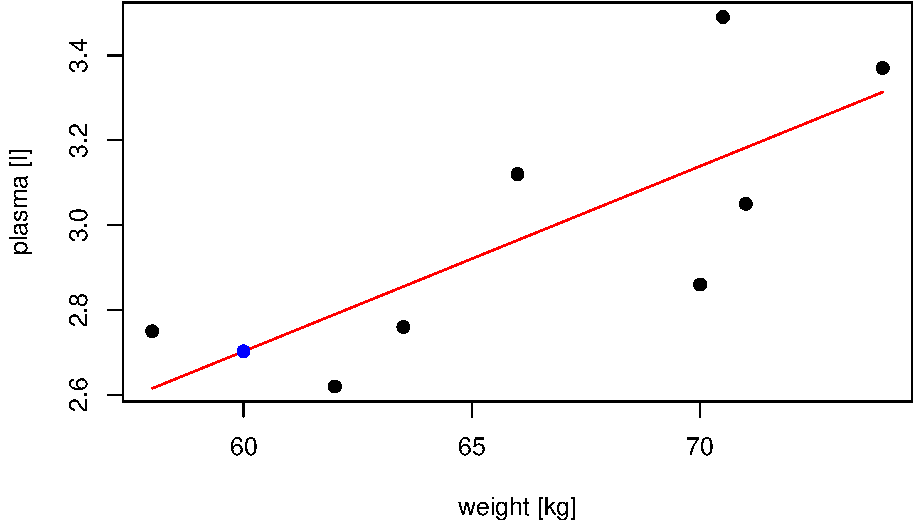
\includegraphics{301-linear-models_files/figure-latex/predict-1.pdf}

\begin{center}\rule{0.5\linewidth}{0.5pt}\end{center}

\hypertarget{exercises-linear-models-i}{%
\section{Exercises: linear models I}\label{exercises-linear-models-i}}

\begin{exercise}
\protect\hypertarget{exr:lm-recognize}{}{\label{exr:lm-recognize} }Linear models form

Which of the following models are linear models and why?

\begin{enumerate}
\def\labelenumi{\alph{enumi})}
\tightlist
\item
  \(Y_i=\alpha + \beta x_i + \epsilon_i\)
\item
  \(Y_i=\beta_0 + \beta_1 x_{i,1} + \beta_2 x_{i,2} + \epsilon_i\)
\item
  \(Y_i=\alpha + \beta x_i + \gamma x_i^2 + \epsilon_i\)
\item
  \(Y_i=\alpha + \gamma x_i^\beta + \epsilon_i\)
\end{enumerate}
\end{exercise}

\begin{exercise}
\protect\hypertarget{exr:lm-protein}{}{\label{exr:lm-protein} }Protein levels in pregnancy

The researchers were interested whether protein levels in expectant mothers are changing throughout the pregnancy. Observations have been taken on 19 healthy women and each woman was at different stage of pregnancy (gestation).

Assuming linear model:

\begin{itemize}
\tightlist
\item
  \(Y_i = \alpha + \beta x_i + \epsilon_i\), where \(Y_i\) corresponds to protein levels in i-th observation
\end{itemize}

and taking summary statisitcs:

\begin{itemize}
\tightlist
\item
  \(\sum_{i=1}^{n}x_i = 456\)
\item
  \(\sum_{i=1}^{n}x_i^2 = 12164\)
\item
  \(\sum_{i=1}^{n}x_iy_i = 369.87\)
\item
  \(\sum_{i=1}^{n}y_i^2 = 11.55\)
\end{itemize}

\begin{enumerate}
\def\labelenumi{\alph{enumi})}
\tightlist
\item
  find the least square estimates of \(\hat{\alpha}\) and \(\hat{\beta}\)
\item
  knowing that e.s.e(\(\hat{\beta}) = 0.022844\) can we
\end{enumerate}

\begin{itemize}
\item
  \begin{enumerate}
  \def\labelenumi{\roman{enumi})}
  \tightlist
  \item
    reject the null hypothesis that the is no relationship between protein level and gestation, i.e.~perform a hypothesis test to test \(H_0:\beta = 0\);
  \end{enumerate}
\item
  \begin{enumerate}
  \def\labelenumi{\roman{enumi})}
  \setcounter{enumi}{1}
  \tightlist
  \item
    can we reject the null hypothesis that \(\beta = 0.02\), i.e.~perform a hypothesis test to test \(H_0:\beta = 0.02\)
  \end{enumerate}
\end{itemize}

\begin{enumerate}
\def\labelenumi{\alph{enumi})}
\setcounter{enumi}{2}
\tightlist
\item
  write down the linear model in the vector-matrix notation and identify response, parameter, design and error matrices
\item
  read in ``protein.csv'' data into R, set Y as protein (response) and calculate using matrix functions the least squares estimates of model coefficients
\item
  use \texttt{lm()} function in R to check your calculations
\item
  use the fitted model in R to predict the value of protein levels at week 20. Try plotting the data, fitted linear model and the predicted value to assess whether your prediction is to be expected.
\end{enumerate}
\end{exercise}

\begin{exercise}
\protect\hypertarget{exr:lm-potato}{}{\label{exr:lm-potato} }
The glucose level in potatoes depends on their storage time and the relationship is somehow curvilinear as shown below.
As we believe that the quadratic function might describe the relationship, assume linear model in form
\(Y_i = \alpha + \beta x_i + \gamma x_i^2 + \epsilon_i \quad i=1,\dots,n\) where \(n=14\) and

\begin{enumerate}
\def\labelenumi{\alph{enumi})}
\tightlist
\item
  write down the model in vector-matrix notation
\item
  load data to from ``potatoes.csv'' and use least squares estimates for obtain estimates of model coefficients
\item
  perform a hypothesis test to test \(H_0:\gamma=0\); and comment whether there is a significant quadratic relationship
\item
  use \texttt{lm()} function to verify your calculations
\item
  predict glucose concentration at storage time 4 and 16 weeks. Plot the data, the fitted model and the predicted values
\end{enumerate}
\end{exercise}

\begin{figure}

{\centering 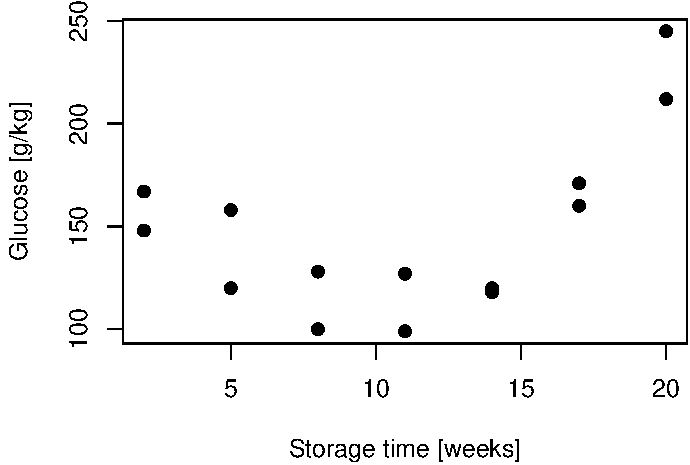
\includegraphics{301-linear-models_files/figure-latex/potatoes-1} 

}

\caption{Sugar in potatoes: relationship between storage time and glucose content}\label{fig:potatoes}
\end{figure}

\hypertarget{answers-to-selected-exercises-linear-models}{%
\section*{Answers to selected exercises (linear models)}\label{answers-to-selected-exercises-linear-models}}
\addcontentsline{toc}{section}{Answers to selected exercises (linear models)}

Exr. \ref{exr:lm-protein}

\begin{enumerate}
\def\labelenumi{\alph{enumi})}
\tightlist
\item
\end{enumerate}

\begin{itemize}
\tightlist
\item
  \(S_{xx} = \sum_{i=1}^{n}x_i^2-\frac{(\sum_{i=1}^{n}x_i)^2}{n}) = 12164 - \frac{456^2}{19} = 1220\)
\item
  \(S_{xy} = \sum_{i=1}^nx_iy_i-\frac{\sum_{i=1}^{n}x_i\sum_{i=1}^{n}y_i}{n} = 369.87 - \frac{(456 \cdot 14.25)}{19} = 27.87\)
\item
  \(\hat{\beta} = \frac{S_{xy}}{S_{xx}} = 27.87 / 1220 = 0.02284\)
\item
  \(\hat{\alpha} = \bar{y}-\frac{S_{xy}}{S_{xx}}\cdot \bar{x} = \frac{14.25}{19}-\frac{27.87}{1220}\cdot \frac{456}{19} = 0.20174\)
\end{itemize}

\begin{enumerate}
\def\labelenumi{\alph{enumi})}
\setcounter{enumi}{1}
\item
  \begin{enumerate}
  \def\labelenumii{\roman{enumii}.}
  \tightlist
  \item
  \end{enumerate}
\end{enumerate}

We can calculate test statistics following:

\begin{itemize}
\tightlist
\item
  \(\frac{\hat{\beta} - \beta}{e.s.e(\hat{\beta})} \sim t(n-p) = \frac{0.02284 - 0}{0.20174} = 6.934\) where the value follows Student's t distribution with \(n-p = 19 - 2 = 17\) degrees of freedom. We can now estimate the a p-value using Student's t distribution table or use R function
\end{itemize}

\begin{Shaded}
\begin{Highlighting}[]
\DecValTok{2}\OperatorTok{*}\KeywordTok{pt}\NormalTok{(}\FloatTok{6.934}\NormalTok{, }\DataTypeTok{df=}\DecValTok{17}\NormalTok{, }\DataTypeTok{lower=}\NormalTok{F)}
\CommentTok{\#\# [1] 2.414315e{-}06}
\end{Highlighting}
\end{Shaded}

As p-value \textless\textless{} 0.001 there is sufficient evidence to reject \(H_0\) in favor of \(H_1\), thus we can conclude that there is a significant relationship between protein levels and gestation

\begin{enumerate}
\def\labelenumi{\alph{enumi})}
\setcounter{enumi}{1}
\item
  \begin{enumerate}
  \def\labelenumii{\roman{enumii}.}
  \setcounter{enumii}{1}
  \tightlist
  \item
  \end{enumerate}
\end{enumerate}

Similarly, we can test \(H_0:\beta = 0.02\), i.e.~\(\frac{\hat{\beta} - \beta}{e.s.e(\hat{\beta})} \sim t(n-p) = \frac{0.02284 - 0.02}{0.20174} = 0.01407753\). Now the test statistics is small

\begin{Shaded}
\begin{Highlighting}[]
\DecValTok{2}\OperatorTok{*}\KeywordTok{pt}\NormalTok{(}\FloatTok{0.01407753}\NormalTok{, }\DataTypeTok{df=}\DecValTok{17}\NormalTok{, }\DataTypeTok{lower=}\NormalTok{F)}
\CommentTok{\#\# [1] 0.988932}
\end{Highlighting}
\end{Shaded}

p-value is large and hence there is no sufficient evidence to reject \(H_0\) and we can conclude that \(\beta = 0.02\)

\begin{enumerate}
\def\labelenumi{\alph{enumi})}
\setcounter{enumi}{2}
\tightlist
\item
  We can rewrite the linear model in vector-matrix formation as \(\mathbf{Y}= \mathbf{\beta}\mathbf{X} + \mathbf{\epsilon}\) where:
\end{enumerate}

response \(\mathbf{Y}=\begin{bmatrix}  y_1 \\  y_2 \\  \vdots \\  y_{19} \end{bmatrix}\)

parameters \(\boldsymbol\beta=\begin{bmatrix}  \alpha \\  \beta \end{bmatrix}\)

design matrix \(\mathbf{X}=\begin{bmatrix}  1 & x_1 \\  1 & x_2 \\  \vdots & \vdots \\  1 & x_{19} \end{bmatrix}\)

errors \(\boldsymbol\epsilon=\begin{bmatrix}  \epsilon_1 \\  \epsilon_2 \\  \vdots \\  \epsilon_{19} \end{bmatrix}\)

\begin{enumerate}
\def\labelenumi{\alph{enumi})}
\setcounter{enumi}{3}
\tightlist
\item
  The least squares estimates in vector-matrix notation is \(\hat{\boldsymbol\beta}= (\mathbf{X}^T\mathbf{X})^{-1}\mathbf{X}^T\mathbf{Y}\) and we can calculate this in R
\end{enumerate}

\begin{Shaded}
\begin{Highlighting}[]
\CommentTok{\# read in data }
\NormalTok{data.protein \textless{}{-}}\StringTok{ }\KeywordTok{read.csv}\NormalTok{(}\StringTok{"data/lm/protein.csv"}\NormalTok{)}

\CommentTok{\# print out top observations}
\KeywordTok{head}\NormalTok{(data.protein)}
\CommentTok{\#\#   Protein Gestation}
\CommentTok{\#\# 1    0.38        11}
\CommentTok{\#\# 2    0.58        12}
\CommentTok{\#\# 3    0.51        13}
\CommentTok{\#\# 4    0.38        15}
\CommentTok{\#\# 5    0.58        17}
\CommentTok{\#\# 6    0.67        18}

\CommentTok{\# define Y and X matrices given the data}
\NormalTok{n \textless{}{-}}\StringTok{ }\KeywordTok{nrow}\NormalTok{(data.protein) }\CommentTok{\# nu. of observations}
\NormalTok{Y \textless{}{-}}\StringTok{  }\KeywordTok{as.matrix}\NormalTok{(data.protein}\OperatorTok{$}\NormalTok{Protein, }\DataTypeTok{ncol=}\DecValTok{1}\NormalTok{) }\CommentTok{\# response }
\NormalTok{X \textless{}{-}}\StringTok{  }\KeywordTok{as.matrix}\NormalTok{(}\KeywordTok{cbind}\NormalTok{(}\KeywordTok{rep}\NormalTok{(}\DecValTok{1}\NormalTok{, }\DataTypeTok{length=}\NormalTok{n), data.protein}\OperatorTok{$}\NormalTok{Gestation)) }\CommentTok{\# design matrix}
\KeywordTok{head}\NormalTok{(X) }\CommentTok{\# double check that the design matrix looks like it should}
\CommentTok{\#\#      [,1] [,2]}
\CommentTok{\#\# [1,]    1   11}
\CommentTok{\#\# [2,]    1   12}
\CommentTok{\#\# [3,]    1   13}
\CommentTok{\#\# [4,]    1   15}
\CommentTok{\#\# [5,]    1   17}
\CommentTok{\#\# [6,]    1   18}

\CommentTok{\# least squares estimate}
\NormalTok{beta.hat \textless{}{-}}\StringTok{ }\KeywordTok{solve}\NormalTok{(}\KeywordTok{t}\NormalTok{(X)}\OperatorTok{\%*\%}\NormalTok{X)}\OperatorTok{\%*\%}\KeywordTok{t}\NormalTok{(X)}\OperatorTok{\%*\%}\NormalTok{Y }\CommentTok{\# beta.hat is a matrix that contains our alpha and beta in the model}
\KeywordTok{print}\NormalTok{(beta.hat)}
\CommentTok{\#\#            [,1]}
\CommentTok{\#\# [1,] 0.20173770}
\CommentTok{\#\# [2,] 0.02284426}
\end{Highlighting}
\end{Shaded}

\begin{enumerate}
\def\labelenumi{\alph{enumi})}
\setcounter{enumi}{4}
\tightlist
\item
  We use \texttt{lm()} function to check our calculations
\end{enumerate}

\begin{Shaded}
\begin{Highlighting}[]
\CommentTok{\# fit linear regression model and print model summary}
\NormalTok{protein \textless{}{-}}\StringTok{ }\NormalTok{data.protein}\OperatorTok{$}\NormalTok{Protein }\CommentTok{\# our Y}
\NormalTok{gestation \textless{}{-}}\StringTok{ }\NormalTok{data.protein}\OperatorTok{$}\NormalTok{Gestation }\CommentTok{\# our X}

\NormalTok{model \textless{}{-}}\StringTok{ }\KeywordTok{lm}\NormalTok{(protein }\OperatorTok{\textasciitilde{}}\StringTok{ }\NormalTok{gestation)}
\KeywordTok{print}\NormalTok{(}\KeywordTok{summary}\NormalTok{(model))}
\CommentTok{\#\# }
\CommentTok{\#\# Call:}
\CommentTok{\#\# lm(formula = protein \textasciitilde{} gestation)}
\CommentTok{\#\# }
\CommentTok{\#\# Residuals:}
\CommentTok{\#\#      Min       1Q   Median       3Q      Max }
\CommentTok{\#\# {-}0.16853 {-}0.08720 {-}0.01009  0.08578  0.20422 }
\CommentTok{\#\# }
\CommentTok{\#\# Coefficients:}
\CommentTok{\#\#             Estimate Std. Error t value Pr(\textgreater{}|t|)    }
\CommentTok{\#\# (Intercept) 0.201738   0.083363   2.420    0.027 *  }
\CommentTok{\#\# gestation   0.022844   0.003295   6.934 2.42e{-}06 ***}
\CommentTok{\#\# {-}{-}{-}}
\CommentTok{\#\# Signif. codes:  0 \textquotesingle{}***\textquotesingle{} 0.001 \textquotesingle{}**\textquotesingle{} 0.01 \textquotesingle{}*\textquotesingle{} 0.05 \textquotesingle{}.\textquotesingle{} 0.1 \textquotesingle{} \textquotesingle{} 1}
\CommentTok{\#\# }
\CommentTok{\#\# Residual standard error: 0.1151 on 17 degrees of freedom}
\CommentTok{\#\# Multiple R{-}squared:  0.7388,	Adjusted R{-}squared:  0.7234 }
\CommentTok{\#\# F{-}statistic: 48.08 on 1 and 17 DF,  p{-}value: 2.416e{-}06}
\end{Highlighting}
\end{Shaded}

\begin{enumerate}
\def\labelenumi{\alph{enumi})}
\setcounter{enumi}{5}
\tightlist
\item
\end{enumerate}

\begin{Shaded}
\begin{Highlighting}[]
\NormalTok{new.obs \textless{}{-}}\StringTok{ }\KeywordTok{data.frame}\NormalTok{(}\DataTypeTok{gestation =} \DecValTok{20}\NormalTok{)}
\NormalTok{y.pred \textless{}{-}}\StringTok{ }\KeywordTok{predict}\NormalTok{(model, }\DataTypeTok{newdata =}\NormalTok{ new.obs)}

\CommentTok{\# we can visualize the data, fitted linear model (red), and the predicted value (blue)}
\KeywordTok{plot}\NormalTok{(gestation, protein, }\DataTypeTok{pch=}\DecValTok{19}\NormalTok{, }\DataTypeTok{xlab=}\StringTok{"gestation [weeks]"}\NormalTok{, }\DataTypeTok{ylab=}\StringTok{"protein levels [mgml{-}1]"}\NormalTok{)}
\KeywordTok{lines}\NormalTok{(gestation, model}\OperatorTok{$}\NormalTok{fitted.values, }\DataTypeTok{col=}\StringTok{"red"}\NormalTok{)}
\KeywordTok{points}\NormalTok{(new.obs, y.pred, }\DataTypeTok{col=}\StringTok{"blue"}\NormalTok{, }\DataTypeTok{pch=}\DecValTok{19}\NormalTok{, }\DataTypeTok{cex =} \DecValTok{1}\NormalTok{)}
\end{Highlighting}
\end{Shaded}

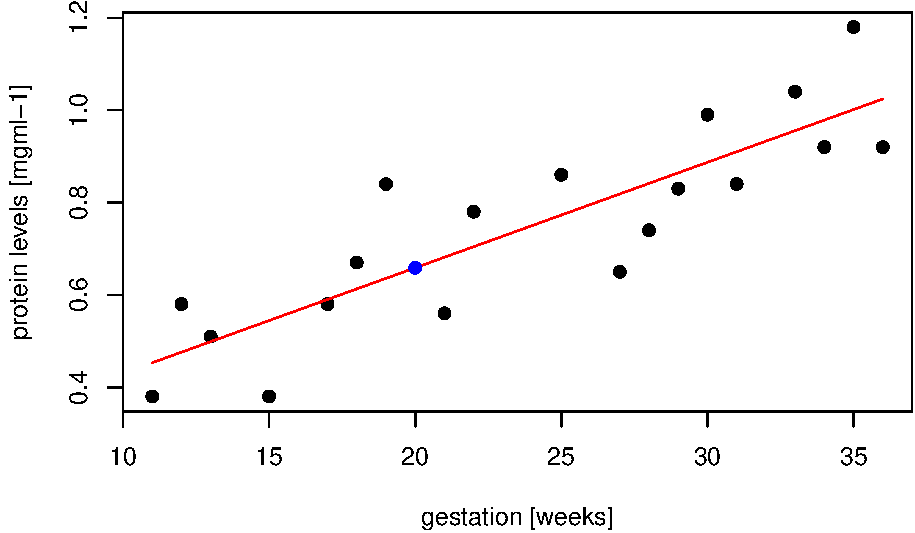
\includegraphics{301-linear-models_files/figure-latex/protein-predict-1.pdf}

Exr. \ref{exr:lm-potato}

\begin{enumerate}
\def\labelenumi{\alph{enumi})}
\tightlist
\item
  We can rewrite the linear model in vector-matrix formation as \(\mathbf{Y}= \boldsymbol\beta\mathbf{X} + \mathbf{\epsilon}\) where:
\end{enumerate}

response \(\mathbf{Y}=\begin{bmatrix}  y_1 \\  y_2 \\  \vdots \\  y_{14} \end{bmatrix}\)

parameters \(\boldsymbol\beta=\begin{bmatrix}  \alpha \\  \beta \\  \gamma \end{bmatrix}\)

design matrix \(\mathbf{X}=\begin{bmatrix}  1 & x_1 & x_1^2\\  1 & x_2 & x_2^2\\  \vdots & \vdots & \vdots \\  1 & x_{14} & x_{14}^2 \end{bmatrix}\)

errors \(\boldsymbol\epsilon=\begin{bmatrix}  \epsilon_1 \\  \epsilon_2 \\  \vdots \\  \epsilon_{14} \end{bmatrix}\)

\begin{enumerate}
\def\labelenumi{\alph{enumi})}
\setcounter{enumi}{1}
\tightlist
\item
  load data to from ``potatoes.csv'' and use least squares estimates for obtain estimates of model coefficients
\end{enumerate}

\begin{Shaded}
\begin{Highlighting}[]
\NormalTok{data.potatoes \textless{}{-}}\StringTok{ }\KeywordTok{read.csv}\NormalTok{(}\StringTok{"data/lm/potatoes.csv"}\NormalTok{)}

\CommentTok{\# define matrices}
\NormalTok{n \textless{}{-}}\StringTok{ }\KeywordTok{nrow}\NormalTok{(data.potatoes)}
\NormalTok{Y \textless{}{-}}\StringTok{  }\NormalTok{data.potatoes}\OperatorTok{$}\NormalTok{Glucose}
\NormalTok{X1 \textless{}{-}}\StringTok{ }\NormalTok{data.potatoes}\OperatorTok{$}\NormalTok{Weeks}
\NormalTok{X2 \textless{}{-}}\StringTok{ }\NormalTok{(data.potatoes}\OperatorTok{$}\NormalTok{Weeks)}\OperatorTok{\^{}}\DecValTok{2}
\NormalTok{X \textless{}{-}}\StringTok{ }\KeywordTok{cbind}\NormalTok{(}\KeywordTok{rep}\NormalTok{(}\DecValTok{1}\NormalTok{, }\KeywordTok{length}\NormalTok{(n)), X1, X2)}
\NormalTok{X \textless{}{-}}\StringTok{ }\KeywordTok{as.matrix}\NormalTok{(X)}

\CommentTok{\# least squares estimate}
\CommentTok{\# beta here refers to the matrix of model coefficients incl. alpha, beta and gamma}
\NormalTok{beta.hat \textless{}{-}}\StringTok{ }\KeywordTok{solve}\NormalTok{(}\KeywordTok{t}\NormalTok{(X)}\OperatorTok{\%*\%}\NormalTok{X)}\OperatorTok{\%*\%}\KeywordTok{t}\NormalTok{(X)}\OperatorTok{\%*\%}\NormalTok{Y }
\KeywordTok{print}\NormalTok{(beta.hat)}
\CommentTok{\#\#          [,1]}
\CommentTok{\#\#    200.169312}
\CommentTok{\#\# X1 {-}19.443122}
\CommentTok{\#\# X2   1.030423}
\end{Highlighting}
\end{Shaded}

\begin{enumerate}
\def\labelenumi{\alph{enumi})}
\setcounter{enumi}{2}
\tightlist
\item
  we use \texttt{lm()} function to verify our calculations:
\end{enumerate}

\begin{Shaded}
\begin{Highlighting}[]
\NormalTok{model \textless{}{-}}\StringTok{ }\KeywordTok{lm}\NormalTok{(Y }\OperatorTok{\textasciitilde{}}\StringTok{ }\NormalTok{X1 }\OperatorTok{+}\StringTok{ }\NormalTok{X2)}
\KeywordTok{print}\NormalTok{(}\KeywordTok{summary}\NormalTok{(model))}
\end{Highlighting}
\end{Shaded}

\begin{verbatim}
## 
## Call:
## lm(formula = Y ~ X1 + X2)
## 
## Residuals:
##     Min      1Q  Median      3Q     Max 
## -17.405 -11.250  -8.071  12.911  29.286 
## 
## Coefficients:
##             Estimate Std. Error t value Pr(>|t|)    
## (Intercept) 200.1693    15.0527  13.298 4.02e-08 ***
## X1          -19.4431     3.1780  -6.118 7.54e-05 ***
## X2            1.0304     0.1406   7.329 1.49e-05 ***
## ---
## Signif. codes:  0 '***' 0.001 '**' 0.01 '*' 0.05 '.' 0.1 ' ' 1
## 
## Residual standard error: 16.4 on 11 degrees of freedom
## Multiple R-squared:  0.8694,	Adjusted R-squared:  0.8457 
## F-statistic: 36.61 on 2 and 11 DF,  p-value: 1.373e-05
\end{verbatim}

\begin{enumerate}
\def\labelenumi{\alph{enumi})}
\setcounter{enumi}{3}
\tightlist
\item
  perform a hypothesis test to test \(H_0:\gamma=0\); and comment whether we there is a significant quadratic term
\end{enumerate}

\begin{itemize}
\tightlist
\item
  \(\frac{\hat{\gamma} - \gamma}{e.s.e(\hat{\gamma})} \sim t(n-p) = \frac{1.030423 - 0}{0.1406} = 7.328755\) where the value follows Student's t distribution with \(n-p = 19 - 2 = 17\) degrees of freedom. We can now estimate the a p-value using Student's t distribution table or use a function in R
\end{itemize}

\begin{Shaded}
\begin{Highlighting}[]
\DecValTok{2}\OperatorTok{*}\KeywordTok{pt}\NormalTok{(}\FloatTok{7.328755}\NormalTok{, }\DataTypeTok{df=}\DecValTok{14{-}3}\NormalTok{, }\DataTypeTok{lower=}\NormalTok{F)}
\CommentTok{\#\# [1] 1.487682e{-}05}
\end{Highlighting}
\end{Shaded}

As p-value \textless\textless{} 0.001 there is sufficient evidence to reject \(H_0\) in favor of \(H_1\), thus we can conclude that there is a significant quadratic relationship between glucose and storage time

\begin{enumerate}
\def\labelenumi{\alph{enumi})}
\setcounter{enumi}{4}
\tightlist
\item
  predict glucose concentration at storage time 4 and 16 weeks
\end{enumerate}

\begin{Shaded}
\begin{Highlighting}[]
\NormalTok{new.obs \textless{}{-}}\StringTok{ }\KeywordTok{data.frame}\NormalTok{(}\DataTypeTok{X1 =} \KeywordTok{c}\NormalTok{(}\DecValTok{4}\NormalTok{, }\DecValTok{16}\NormalTok{), }\DataTypeTok{X2 =} \KeywordTok{c}\NormalTok{(}\DecValTok{4}\OperatorTok{\^{}}\DecValTok{2}\NormalTok{, }\DecValTok{16}\OperatorTok{\^{}}\DecValTok{2}\NormalTok{))}
\NormalTok{pred.y \textless{}{-}}\StringTok{ }\KeywordTok{predict}\NormalTok{(model, }\DataTypeTok{newdata =}\NormalTok{ new.obs)}

\KeywordTok{plot}\NormalTok{(data.potatoes}\OperatorTok{$}\NormalTok{Weeks, data.potatoes}\OperatorTok{$}\NormalTok{Glucose, }\DataTypeTok{xlab=}\StringTok{"Storage time [weeks]"}\NormalTok{, }\DataTypeTok{ylab=}\StringTok{"Glucose [g/kg]"}\NormalTok{, }\DataTypeTok{pch=}\DecValTok{19}\NormalTok{)}
\KeywordTok{lines}\NormalTok{(data.potatoes}\OperatorTok{$}\NormalTok{Weeks, model}\OperatorTok{$}\NormalTok{fitted.values, }\DataTypeTok{col=}\StringTok{"red"}\NormalTok{)}
\KeywordTok{points}\NormalTok{(new.obs[,}\DecValTok{1}\NormalTok{], pred.y, }\DataTypeTok{pch=}\DecValTok{19}\NormalTok{, }\DataTypeTok{col=}\StringTok{"blue"}\NormalTok{)}
\end{Highlighting}
\end{Shaded}

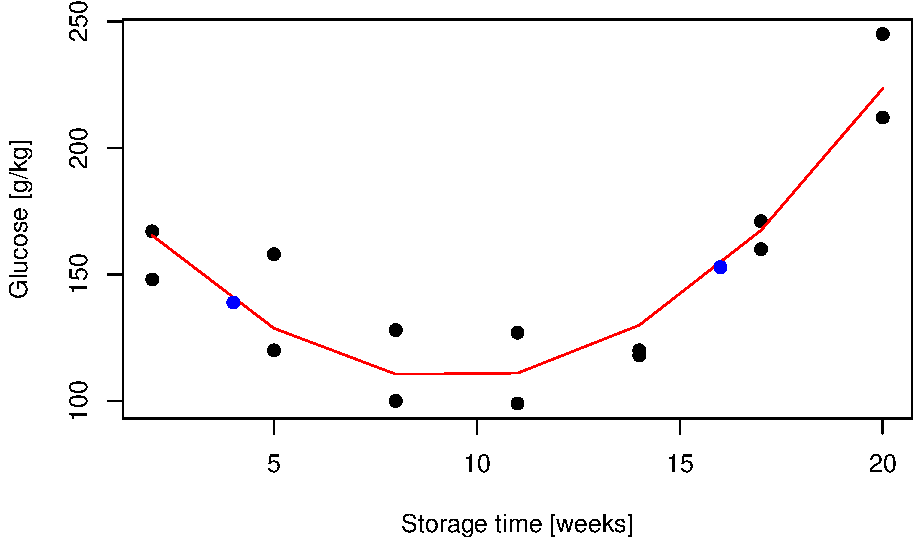
\includegraphics{301-linear-models_files/figure-latex/potato-predict-1.pdf}

\hypertarget{interpreting-regression-coefficients}{%
\chapter{Interpreting regression coefficients}\label{interpreting-regression-coefficients}}

\textbf{Aims}

\begin{itemize}
\tightlist
\item
  xxx
\end{itemize}

\textbf{Learning outcomes}

\begin{itemize}
\tightlist
\item
  xxx
\end{itemize}

\hypertarget{model-assumptions}{%
\chapter{Model assumptions}\label{model-assumptions}}

\textbf{Aims}

\begin{itemize}
\tightlist
\item
  xxx
\end{itemize}

\textbf{Learning outcomes}

\begin{itemize}
\tightlist
\item
  xxx
\end{itemize}

\hypertarget{generalized-linear-models}{%
\chapter{Generalized linear models}\label{generalized-linear-models}}

\textbf{Aims}

\begin{itemize}
\tightlist
\item
  xxx
\end{itemize}

\textbf{Learning outcomes}

\begin{itemize}
\tightlist
\item
  xxx
\end{itemize}

\hypertarget{linear-mixed-models}{%
\chapter{Linear Mixed Models}\label{linear-mixed-models}}

\textbf{Aims}

\begin{itemize}
\tightlist
\item
  xxx
\end{itemize}

\textbf{Learning outcomes}

\begin{itemize}
\tightlist
\item
  xxx
\end{itemize}

\end{document}
